\documentclass[12pt,a4paper]{article}

% --- Essential Packages ---
\usepackage[utf8]{inputenc}
\usepackage[T1]{fontenc}
\usepackage{lmodern}
\usepackage[margin=1in,headheight=15pt]{geometry}
\usepackage{graphicx}
\usepackage{xcolor}
\usepackage{listings}
\usepackage{tcolorbox}
\usepackage{fancyhdr}
\usepackage{booktabs}
\usepackage{tabularx}
\usepackage{titlesec}
\usepackage{float}
\usepackage{caption}
\usepackage{enumitem}
\usepackage{hyperref}

% --- Directories for screenshots and images ---
\graphicspath{{./screenshots/}{./images/}}

% --- Color Definitions ---
\definecolor{codegray}{rgb}{0.5,0.5,0.5}
\definecolor{codebg}{RGB}{247,249,251}
\definecolor{sqlkeyword}{RGB}{0,80,180}
\definecolor{sqlstring}{RGB}{180,50,50}
\definecolor{sqlcomment}{RGB}{100,120,130}
\definecolor{accentblue}{RGB}{25,75,140}

% --- Hyperref Setup ---
\hypersetup{
    plainpages=false,
    colorlinks=true,
    linkcolor=accentblue,
    filecolor=magenta,
    urlcolor=accentblue,
    pdftitle={DBMS Practical Record - Jyotirmoy Das},
    pdfauthor={Jyotirmoy Das}
}

% --- Listings / Code Block Style for SQL ---
\lstdefinestyle{sqlstyle}{
    language=SQL,
    backgroundcolor=\color{codebg},
    commentstyle=\color{sqlcomment}\itshape,
    keywordstyle=\color{sqlkeyword}\bfseries,
    numberstyle=\tiny\color{codegray},
    stringstyle=\color{sqlstring},
    basicstyle=\ttfamily\footnotesize,
    breakatwhitespace=false,
    breaklines=true,
    captionpos=b,
    keepspaces=true,
    numbers=left,
    numbersep=8pt,
    showspaces=false,
    showstringspaces=false,
    showtabs=false,
    tabsize=4,
    frame=single,
    rulecolor=\color{black!15},
    morekeywords={
        CREATE, TABLE, DATABASE, USE, DROP, ALTER, ADD, MODIFY,
        SELECT, FROM, WHERE, GROUP, BY, HAVING, ORDER, ASC, DESC,
        INSERT, INTO, VALUES, UPDATE, SET, DELETE,
        PRIMARY, KEY, FOREIGN, REFERENCES, NOT, NULL, UNIQUE, CHECK, DEFAULT,
        JOIN, INNER, LEFT, RIGHT, FULL, ON,
        VARCHAR, INT, FLOAT, DATE, CHAR, DECIMAL, AUTO_INCREMENT, TIMESTAMP
    }
}
\lstset{style=sqlstyle}

% --- Custom Header & Footer ---
\pagestyle{fancy}
\fancyhf{}
\fancyhead[L]{\textsf{\footnotesize Database Management Systems Lab}}
\fancyhead[R]{\textsf{\footnotesize Practical Record}}
\fancyfoot[C]{\thepage}
\renewcommand{\headrulewidth}{0.4pt}
\renewcommand{\footrulewidth}{0.4pt}

% --- Custom callout box ---
\newtcolorbox{infobox}[1][]{
    colback=accentblue!5,
    colframe=accentblue!75,
    fonttitle=\bfseries,
    title=#1,
    boxrule=0.8pt,
    arc=3pt
}

% --- Section formatting ---
\titleformat{\section}{\raggedright\Large\bfseries\color{accentblue}}{\thesection}{1em}{}[\titlerule]
\titlespacing*{\section}{0pt}{10pt plus 2pt minus 2pt}{6pt plus 1pt minus 1pt}
\titlespacing*{\subsection}{0pt}{8pt plus 2pt minus 2pt}{4pt plus 1pt minus 1pt}
\titlespacing*{\subsubsection}{0pt}{6pt plus 1pt minus 1pt}{3pt plus 1pt minus 1pt}

% --- Compact Lists ---
\setlist{noitemsep, topsep=3pt, parsep=0pt, partopsep=0pt}

\begin{document}

% =========================================================================
% COVER PAGE (Departmental Lab Copy Format)
% =========================================================================
\pagenumbering{Alph}
\begin{titlepage}
\begin{center}
    \vspace*{0.2cm}

    % --- Institutional Emblem / Gauhati University Logo ---
    
\includegraphics[height=3.3cm,keepaspectratio]{gu-logo-black.png}\par
    \vspace{0.45cm}

    % --- Department & Institution Header ---
    {\LARGE \textbf{Department of Information Technology}}\\[0.25cm]
    {\large \textit{Gauhati University Institute of Science \& Technology}}\\[0.25cm]
    {\large Gauhati University, Guwahati -- 14}\par

    \vfill

    % --- Lab Copy & Course Title ---
    {\Large --- Lab Copy ---}\\[0.45cm]
    {\Large \textbf{\textit{Database Management Systems Lab (IT 311)}}}\par

    \vfill

    % --- Student Details ---
    {\large \textbf{Name: Jyotirmoy Das}}\\[0.35cm]
    {\large \textbf{Roll No: 240103002}}\\[0.35cm]
    {\large \textbf{Semester: 5\textsuperscript{th} Semester}}\\[0.35cm]
    {\large \textbf{Branch: Computer Science and Engineering}}\par

    \vspace*{1.2cm}
\end{center}
\end{titlepage}

% =========================================================================
% FRONT MATTER (Roman numerals)
% =========================================================================
\pagenumbering{roman}
\setcounter{page}{1}

% --- Laboratory Record Index Page (Template Format) ---
\newpage
\thispagestyle{plain}
\pdfbookmark[0]{Index}{index}

\begin{center}
    {\LARGE \textbf{Database Management Systems (DBMS)}}\\[0.25cm]
    {\Large \textbf{INDEX OF PRACTICAL WORK}}
\end{center}

\vspace{0.4cm}

\noindent\begin{tabular*}{\linewidth}{@{\extracolsep{\fill}}lr@{}}
\textbf{Student Name:} Jyotirmoy Das & \textbf{Roll No.:} 240103002 \\[0.2cm]
\textbf{Programme / Sem.:} B.Tech / 5\textsuperscript{th} Sem. & \textbf{Branch:} Computer Science \& Engg. \\[0.2cm]
\multicolumn{2}{@{}l}{\textbf{Subject:} Database Management Systems (DBMS)}
\end{tabular*}

\vspace{0.4cm}

\renewcommand{\arraystretch}{1.45}
\noindent\begin{tabularx}{\linewidth}{|c|c|>{\raggedright\arraybackslash}X|c|c|}
\hline
\textbf{Sl. No.} & \textbf{Date} & \textbf{Practical Question / Title} & \textbf{Page No.} & \textbf{Faculty Sign} \\ \hline
1 & 06/10/2026 & Experiment 2 (Prob. 1): DDL -- College Database & \pageref{exp:ddl_prob1} & \\ \hline
2 & 06/10/2026 & Experiment 2 (Prob. 2): DDL -- Banking Enterprise & \pageref{exp:ddl_prob2} & \\ \hline
3 & 13/10/2026 & Experiment 3 (Prob. 1): DML -- College Database & \pageref{exp:dml_prob1} & \\ \hline
4 & 13/10/2026 & Experiment 3 (Prob. 2): DML -- Banking Enterprise & \pageref{exp:dml_prob2} & \\ \hline
5 & 20/10/2026 & Experiment 4 (Prob. 1): Subqueries and Joins -- Banking Enterprise & \pageref{exp:subqueries_prob1} & \\ \hline
6 & 20/10/2026 & Experiment 4 (Prob. 2): Subqueries and Joins -- College Database & \pageref{exp:subqueries_prob2} & \\ \hline
7 & & & & \\ \hline
8 & & & & \\ \hline
9 & & & & \\ \hline
10 & & & & \\ \hline
11 & & & & \\ \hline
12 & & & & \\ \hline
13 & & & & \\ \hline
14 & & & & \\ \hline
\end{tabularx}

\newpage

% =========================================================================
% PRACTICALS / EXPERIMENTS (Arabic numbering)
% =========================================================================
\pagenumbering{arabic}

% =========================================================================
% EXPERIMENT 2 - PROBLEM 1: COLLEGE DATABASE DDL
% =========================================================================
\label{exp:ddl}
\label{exp:ddl_prob1}
\noindent
\begin{center}
    {\LARGE \textbf{DBMS LABORATORY PRACTICAL}}\\[0.25cm]
    \textbf{Practical No.:} 2 (Problem 1) \hfill \textbf{Date:} 06/10/2026 \hfill \textbf{Page No.:} \thepage
\end{center}
\vspace{-0.2cm}
\hrule
\vspace{0.35cm}

\subsection*{Question / Problem Statement}
Consider the database for a college. Design and implement the relational database schema using Data Definition Language (DDL) commands in MySQL:
\begin{enumerate}[noitemsep,topsep=2pt]
    \item[(i)] Create the database \texttt{college} and select it as the active database context.
    \item[(ii)] Create the following relational tables with their integrity constraints: \texttt{Department}, \texttt{Student}, \texttt{Faculty}, \texttt{Course}, \texttt{Register}, \texttt{Teaching}, and \texttt{Hostel}.
    \item[(iii)] Enforce primary key, foreign key, not null, unique, check, and default constraints.
    \item[(iv)] Display all tables in the database using \texttt{SHOW TABLES;}.
    \item[(v)] Describe the schema structure of all tables using \texttt{DESCRIBE}.
    \item[(vi)] Modify the \texttt{Student} table to add a new column \texttt{grade CHAR(2)} via \texttt{ALTER TABLE}.
\end{enumerate}

\subsection*{1. Database \& Table Creation with Integrity Constraints}

\subsubsection*{SQL Query}
\begin{lstlisting}[basicstyle=\ttfamily\footnotesize,caption={Creating college database and relational tables with integrity constraints}]
-- Create and select college database
CREATE DATABASE college;
USE college;

-- 1. Department table
CREATE TABLE Department (
    dno INT PRIMARY KEY,
    dname VARCHAR(50) NOT NULL UNIQUE
);

-- 2. Student table (referencing Department)
CREATE TABLE Student (
    sid INT PRIMARY KEY,
    sname VARCHAR(50) NOT NULL,
    sex CHAR(1) CHECK (sex IN ('M', 'F', 'O')),
    dob DATE NOT NULL,
    dno INT,
    FOREIGN KEY (dno) REFERENCES Department(dno)
);

-- 3. Faculty table (referencing Department)
CREATE TABLE Faculty (
    f_id INT PRIMARY KEY,
    fname VARCHAR(50) NOT NULL,
    designation VARCHAR(50) DEFAULT 'Assistant Professor',
    salary DECIMAL(10, 2) CHECK (salary > 0),
    dno INT,
    FOREIGN KEY (dno) REFERENCES Department(dno)
);

-- 4. Course table (referencing Department)
CREATE TABLE Course (
    cid INT PRIMARY KEY,
    cname VARCHAR(50) NOT NULL UNIQUE,
    credits INT CHECK (credits BETWEEN 1 AND 6),
    dno INT,
    FOREIGN KEY (dno) REFERENCES Department(dno)
);

-- 5. Register table (composite primary key and foreign keys)
CREATE TABLE Register (
    sid INT,
    cid INT,
    sem INT DEFAULT 1,
    PRIMARY KEY (sid, cid),
    FOREIGN KEY (sid) REFERENCES Student(sid),
    FOREIGN KEY (cid) REFERENCES Course(cid)
);

-- 6. Teaching table (composite primary key and foreign keys)
CREATE TABLE Teaching (
    f_id INT,
    cid INT,
    sem INT DEFAULT 1,
    PRIMARY KEY (f_id, cid),
    FOREIGN KEY (f_id) REFERENCES Faculty(f_id),
    FOREIGN KEY (cid) REFERENCES Course(cid)
);

-- 7. Hostel table
CREATE TABLE Hostel (
    hid INT PRIMARY KEY,
    hname VARCHAR(50) NOT NULL UNIQUE,
    seats INT DEFAULT 100 CHECK (seats > 0)
);
\end{lstlisting}

\vspace{0.2cm}

\subsection*{2. Schema Inspection \& Dynamic Alteration}

\subsubsection*{SQL Query}
\begin{lstlisting}[basicstyle=\ttfamily\footnotesize,caption={Displaying tables, inspecting schemas, and altering table structure}]
-- Display all created tables in college database
SHOW TABLES;

-- Inspect schema definitions and constraints
DESCRIBE Department;
DESCRIBE Student;
DESCRIBE Faculty;
DESCRIBE Course;
DESCRIBE Register;
DESCRIBE Teaching;
DESCRIBE Hostel;

-- Dynamically alter Student table to add grade column
ALTER TABLE Student ADD COLUMN grade CHAR(2);
\end{lstlisting}

\newpage

\subsection*{Output Screenshots}

\begin{figure}[H]
    \centering
    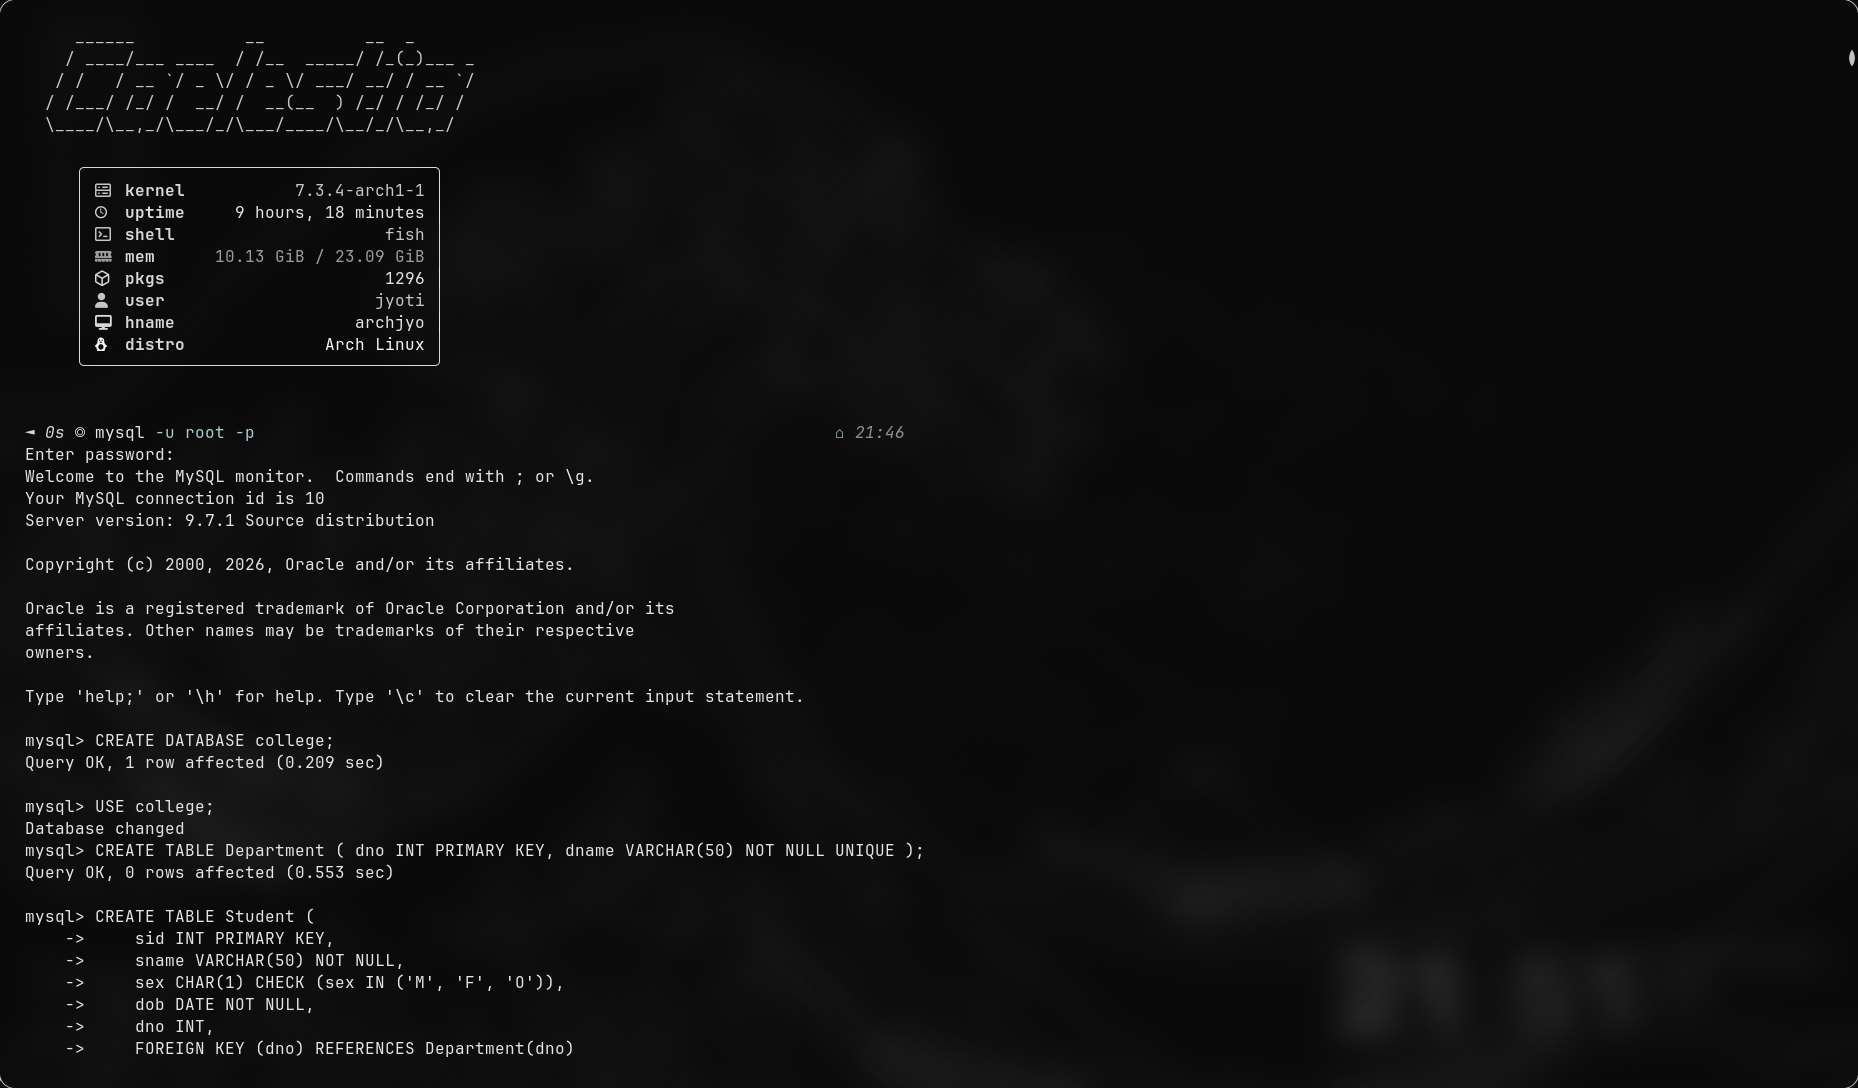
\includegraphics[width=0.92\linewidth,height=7.8cm,keepaspectratio]{Exp2-prob1-1.png}
    \caption{Database creation, active context selection, and Department/Student table creation.}
    \label{fig:exp2_create1}
\end{figure}

\vspace{0.2cm}

\begin{figure}[H]
    \centering
    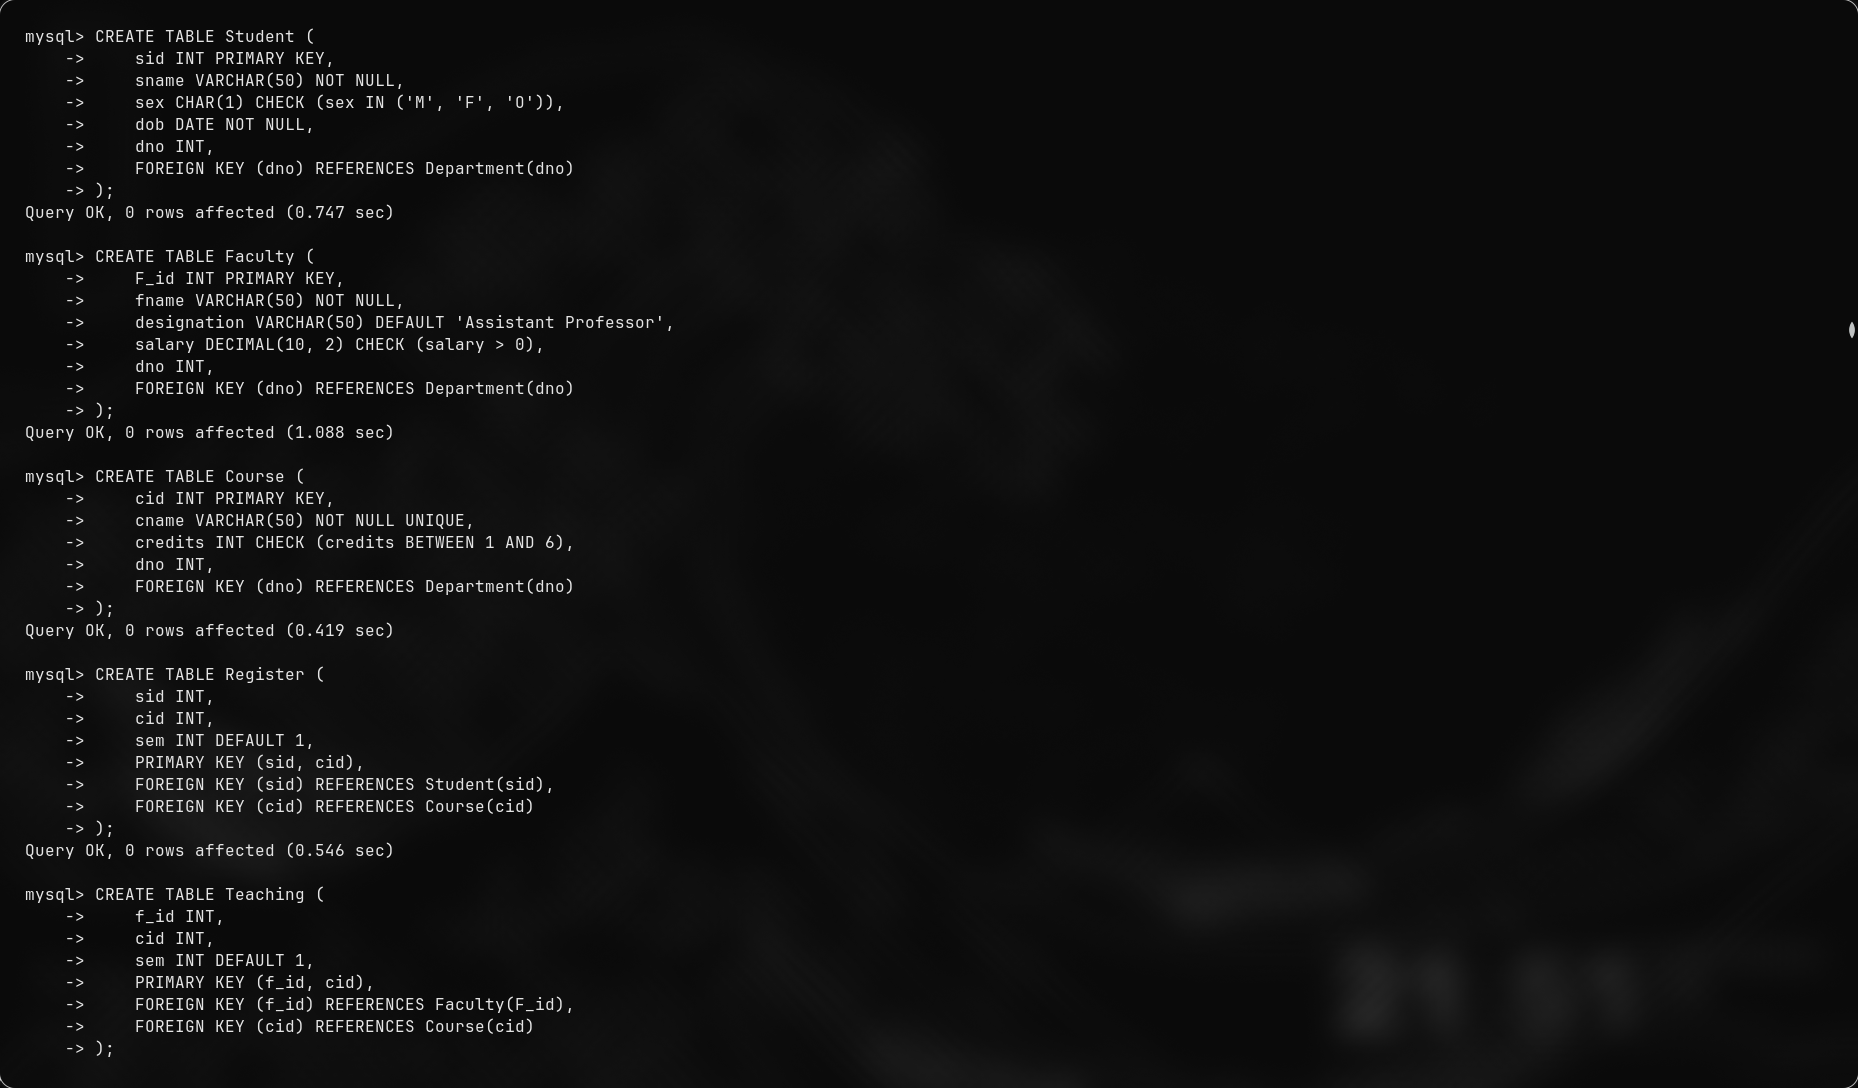
\includegraphics[width=0.92\linewidth,height=8.0cm,keepaspectratio]{Exp2-prob1-2.png}
    \caption{Creation of Student, Faculty, Course, Register, and Teaching tables with constraints.}
    \label{fig:exp2_create2}
\end{figure}

\newpage

\begin{figure}[H]
    \centering
    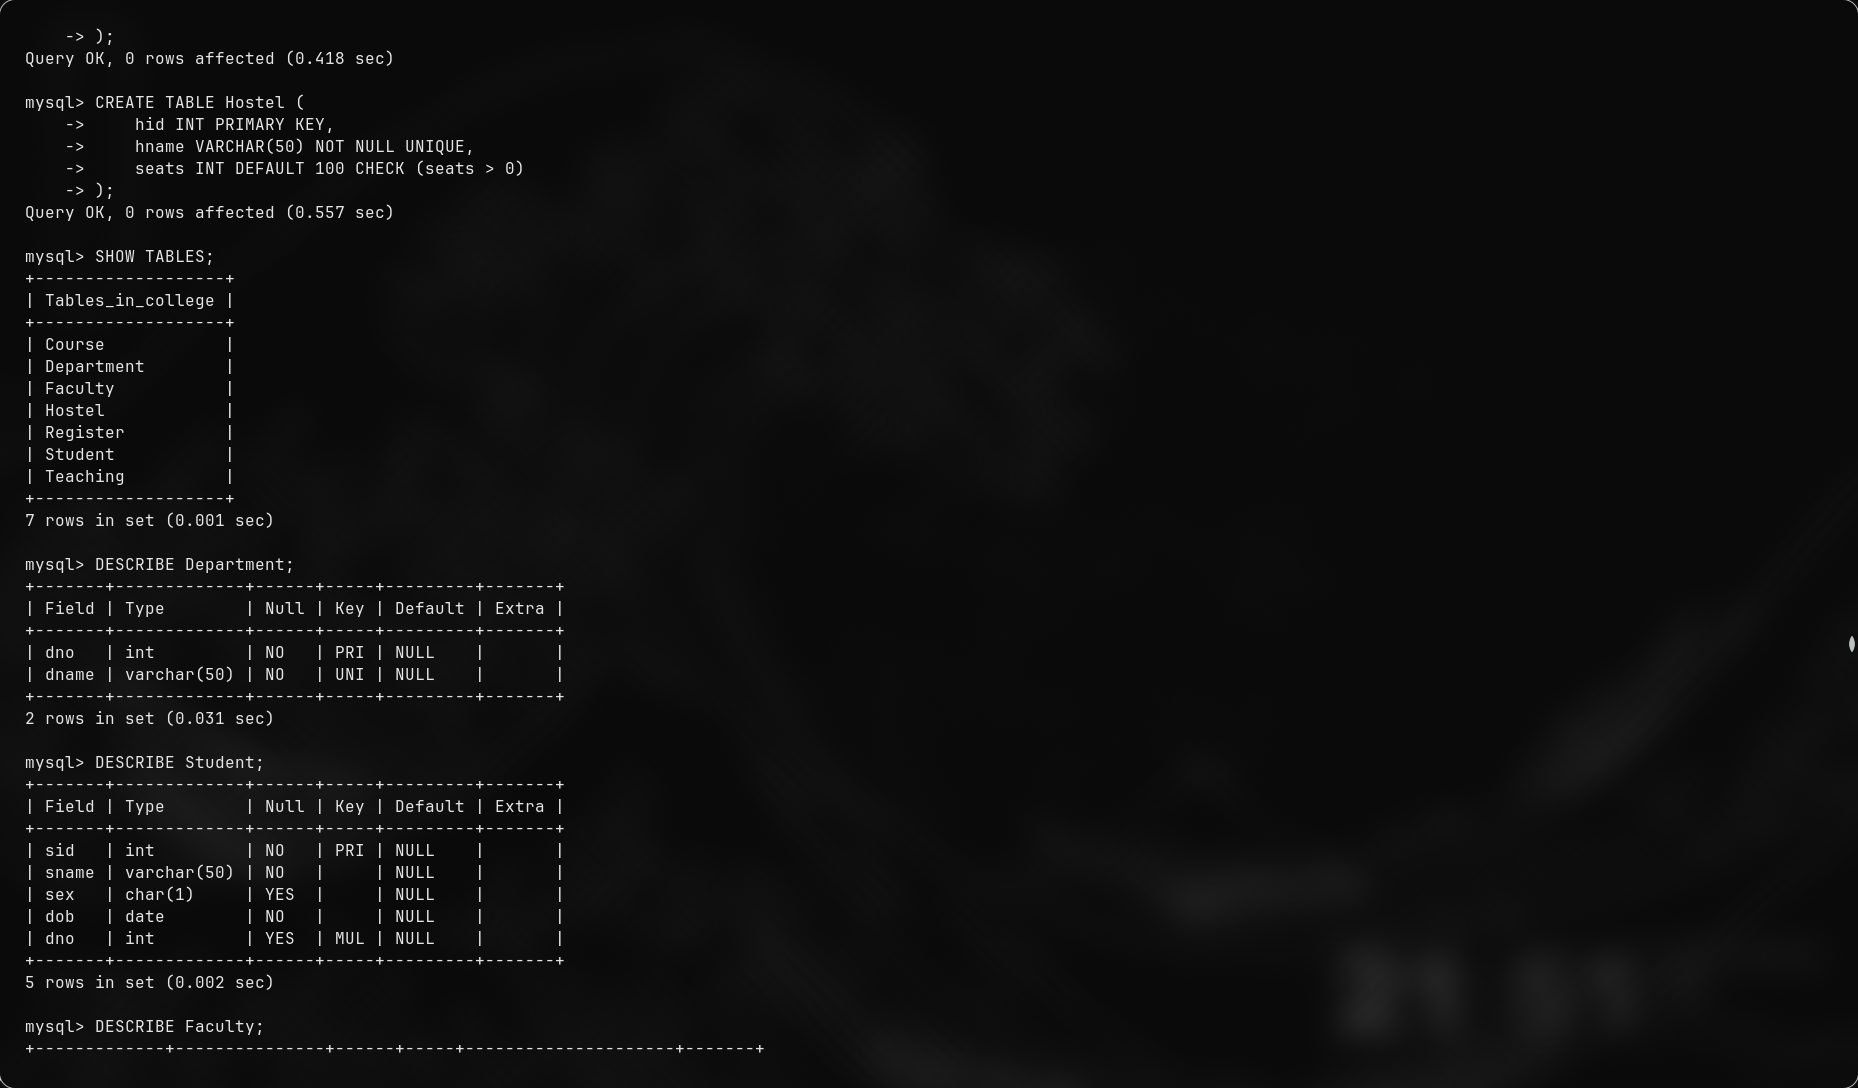
\includegraphics[width=0.92\linewidth,height=7.8cm,keepaspectratio]{Exp2-prob1-3.png}
    \caption{Hostel table creation, table catalog verification, and schema inspection of Department and Student.}
    \label{fig:exp2_inspect1}
\end{figure}

\vspace{0.2cm}

\begin{figure}[H]
    \centering
    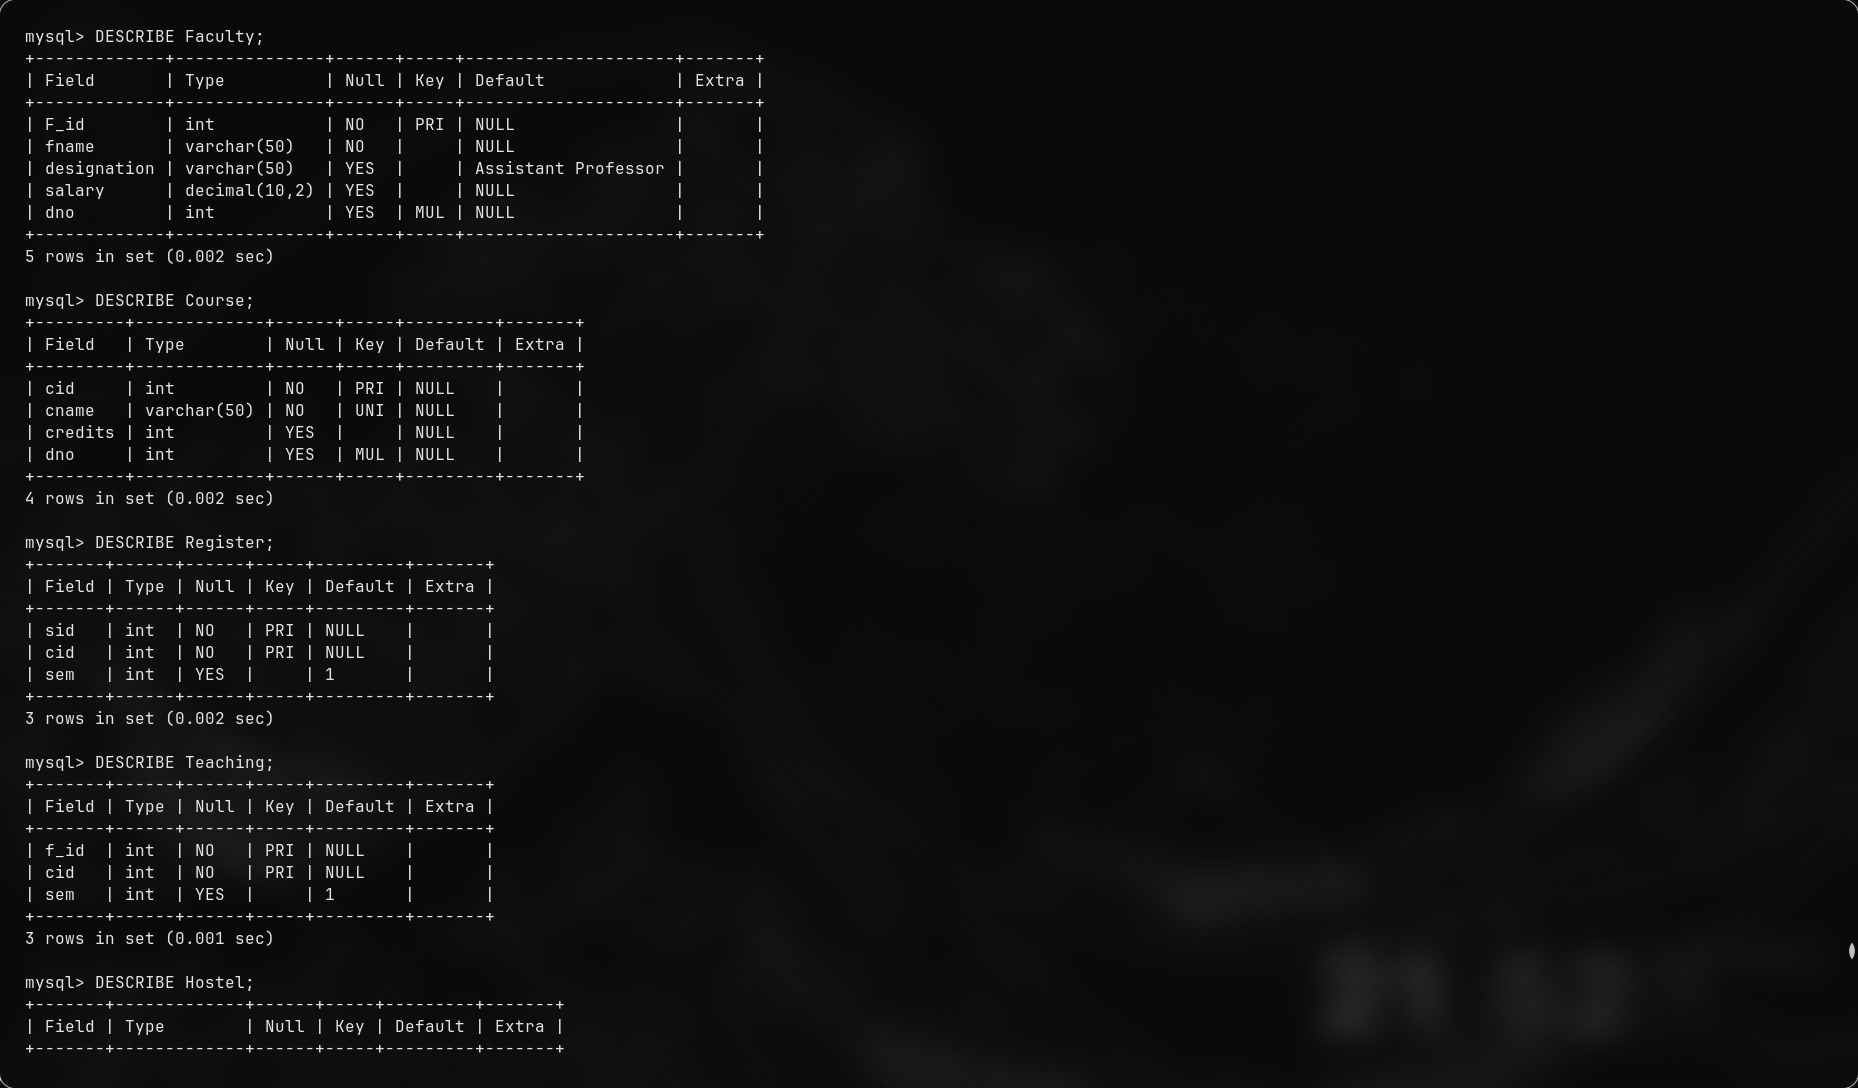
\includegraphics[width=0.92\linewidth,height=8.0cm,keepaspectratio]{Exp2-prob1-4.png}
    \caption{Schema inspection of Faculty, Course, Register, and Teaching tables.}
    \label{fig:exp2_inspect2}
\end{figure}

\newpage

\begin{figure}[H]
    \centering
    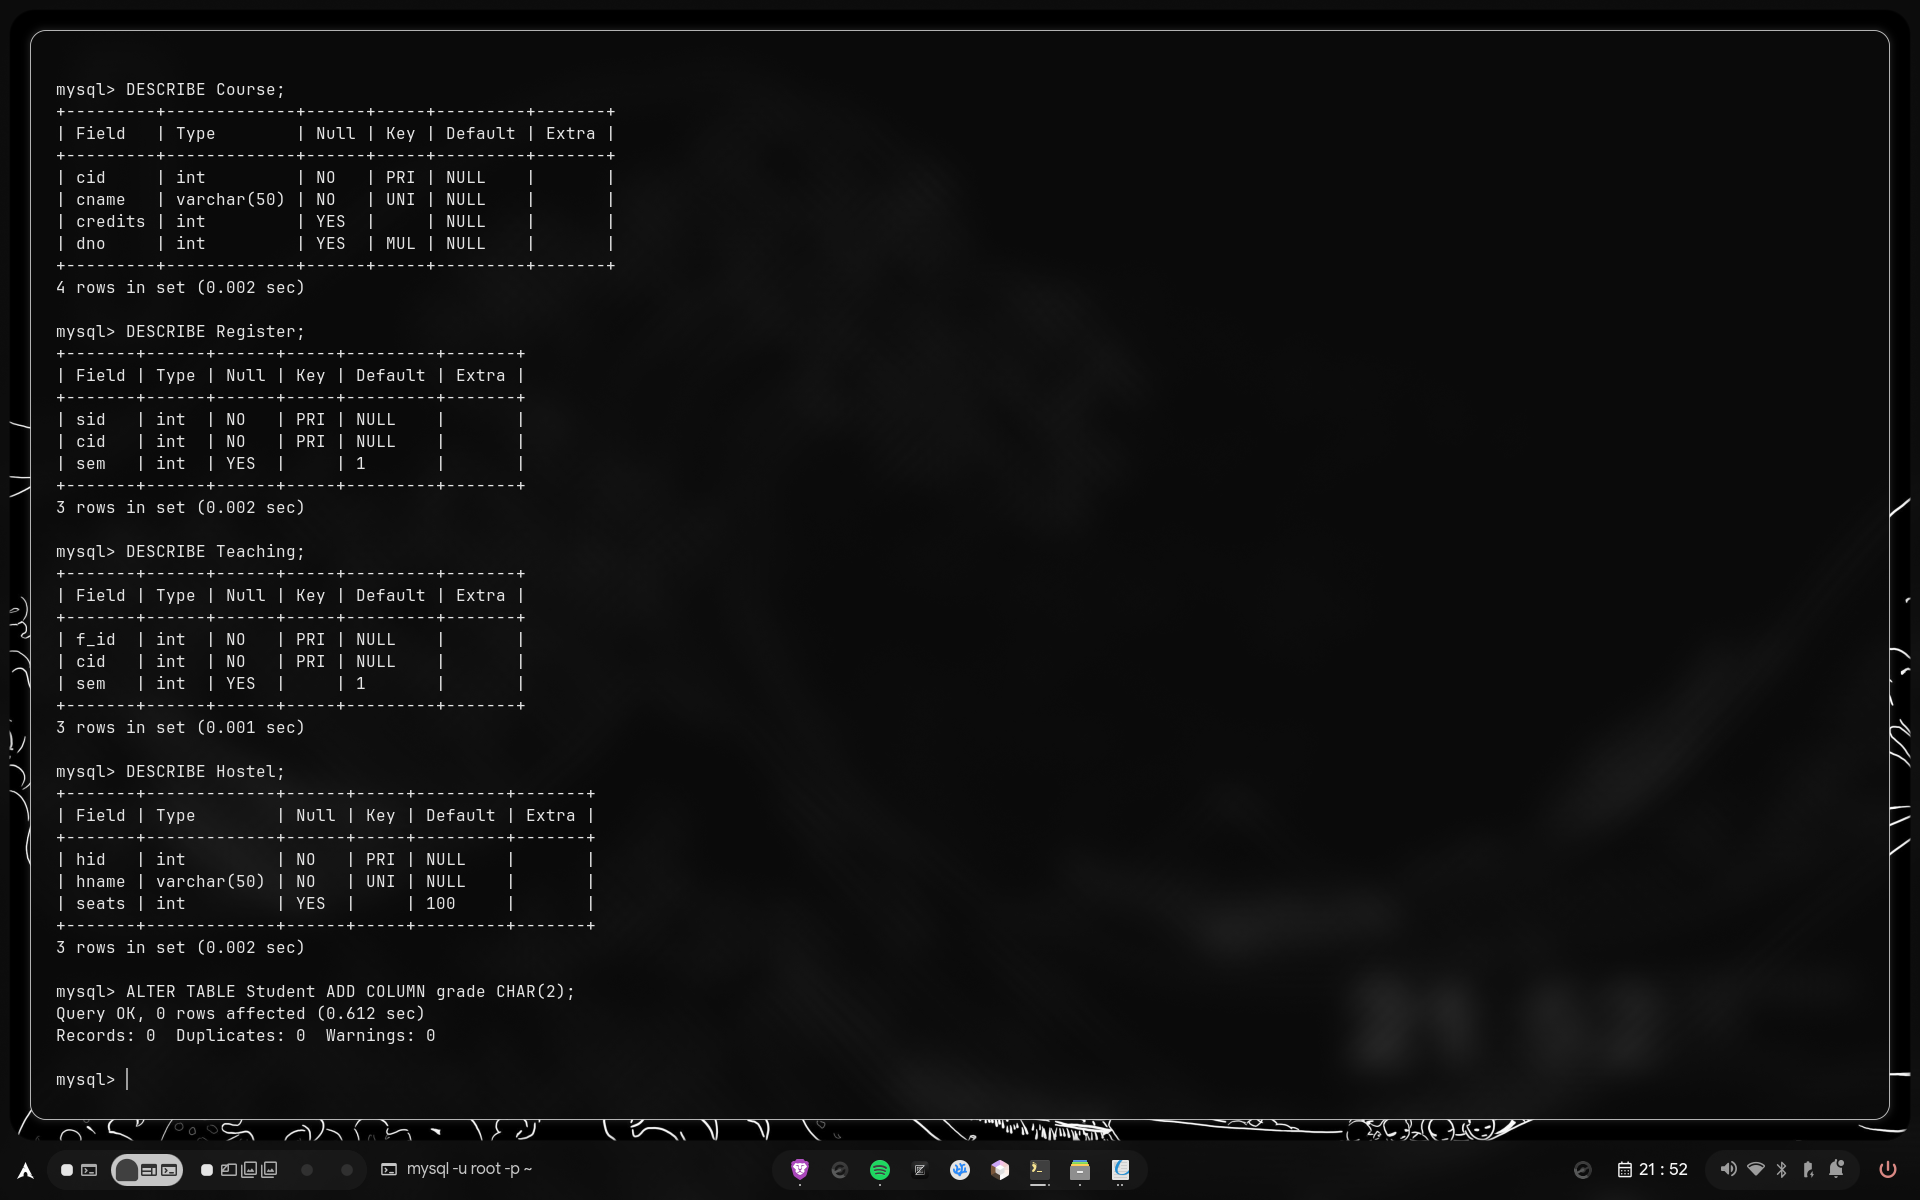
\includegraphics[width=0.92\linewidth,height=9.5cm,keepaspectratio]{Exp2-prob1-5.png}
    \caption{Hostel table schema inspection and dynamic addition of \texttt{grade} column via \texttt{ALTER TABLE}.}
    \label{fig:exp2_alter}
\end{figure}

\vspace{0.4cm}
\noindent\textbf{Result / Observation:}\quad The Data Definition Language (DDL) commands for the College database were executed successfully in MySQL. All relational tables were created with appropriate entity and referential integrity constraints, table schemas were verified via \texttt{DESCRIBE}, and structural modification using \texttt{ALTER TABLE} was confirmed.

\newpage

% =========================================================================
% EXPERIMENT 2 - PROBLEM 2: BANKING ENTERPRISE DATABASE DDL
% =========================================================================
\label{exp:ddl_prob2}
\noindent
\begin{center}
    {\LARGE \textbf{DBMS LABORATORY PRACTICAL}}\\[0.25cm]
    \textbf{Practical No.:} 2 (Problem 2) \hfill \textbf{Date:} 06/10/2026 \hfill \textbf{Page No.:} \thepage
\end{center}
\vspace{-0.2cm}
\hrule
\vspace{0.35cm}

\subsection*{Question / Problem Statement}
Consider the database for a banking enterprise. Design and implement the relational database schema using Data Definition Language (DDL) commands in MySQL:
\begin{enumerate}[noitemsep,topsep=2pt]
    \item[(i)] Create the database \texttt{bank} and select it as the active database context.
    \item[(ii)] Create the following relational tables with their integrity constraints: \texttt{customer}, \texttt{Bank\_brn}, \texttt{Deposit}, \texttt{Loan}, \texttt{Accounts\_in}, \texttt{depositor}, and \texttt{borrower}.
    \item[(iii)] Enforce primary key, foreign key, not null, check, and default constraints.
    \item[(iv)] Display all tables in the database using \texttt{SHOW TABLES;}.
    \item[(v)] Describe the schema structure of all tables using \texttt{DESCRIBE}.
    \item[(vi)] Remove the relational tables from the database using \texttt{DROP TABLE}.
\end{enumerate}

\subsection*{1. Database \& Table Creation with Integrity Constraints}

\subsubsection*{SQL Query}
\begin{lstlisting}[basicstyle=\ttfamily\footnotesize,caption={Creating bank database and relational tables with integrity constraints}]
-- Create and select bank database
CREATE DATABASE bank;
USE bank;

-- 1. customer table
CREATE TABLE customer (
    cid INT PRIMARY KEY,
    cname VARCHAR(50) NOT NULL,
    loc VARCHAR(50) NOT NULL,
    sex CHAR(1) CHECK (sex IN ('M', 'F', 'O')),
    dob DATE NOT NULL
);

-- 2. Bank_brn table
CREATE TABLE Bank_brn (
    bcode INT PRIMARY KEY,
    bloc VARCHAR(50) NOT NULL,
    bsate VARCHAR(50) NOT NULL
);

-- 3. Deposit table
CREATE TABLE Deposit (
    Dacno INT PRIMARY KEY,
    dtype VARCHAR(50) DEFAULT 'Savings',
    ddate DATE NOT NULL,
    damt DECIMAL(10, 2) CHECK (damt >= 0)
);

-- 4. Loan table
CREATE TABLE Loan (
    Lacno INT PRIMARY KEY,
    ltype VARCHAR(30) NOT NULL,
    ldate DATE NOT NULL,
    lamt DECIMAL(12, 2) CHECK (lamt > 0)
);

-- 5. Accounts_in table (composite PK, FK referencing Bank_brn and customer)
CREATE TABLE Accounts_in (
    Bcode INT,
    cid INT,
    PRIMARY KEY (Bcode, cid),
    FOREIGN KEY (Bcode) REFERENCES Bank_brn(bcode),
    FOREIGN KEY (cid) REFERENCES customer(cid)
);

-- 6. depositor table (composite PK, FK referencing customer and Deposit)
CREATE TABLE depositor (
    cid INT,
    dacno INT,
    PRIMARY KEY (cid, dacno),
    FOREIGN KEY (cid) REFERENCES customer(cid),
    FOREIGN KEY (dacno) REFERENCES Deposit(Dacno)
);

-- 7. borrower table (composite PK, FK referencing customer and Loan)
CREATE TABLE borrower (
    cid INT,
    lacno INT,
    PRIMARY KEY (cid, lacno),
    FOREIGN KEY (cid) REFERENCES customer(cid),
    FOREIGN KEY (lacno) REFERENCES Loan(Lacno)
);
\end{lstlisting}

\vspace{0.2cm}

\subsection*{2. Schema Inspection \& Table Destruction Commands}

\subsubsection*{SQL Query}
\begin{lstlisting}[basicstyle=\ttfamily\footnotesize,caption={Inspecting schema definitions and dropping tables}]
-- Display all created tables in bank database
SHOW TABLES;

-- Inspect schema definitions and constraints
DESCRIBE customer;
DESCRIBE Bank_brn;
DESCRIBE Deposit;
DESCRIBE Accounts_in;
DESCRIBE Loan;
DESCRIBE depositor;
DESCRIBE borrower;

-- Drop relational tables in referential integrity order
DROP TABLE borrower;
DROP TABLE depositor;
DROP TABLE Accounts_in;
DROP TABLE Loan;
DROP TABLE Deposit;
DROP TABLE Bank_brn;
DROP TABLE customer;
\end{lstlisting}

\newpage

\subsection*{Output Screenshots}

\begin{figure}[H]
    \centering
    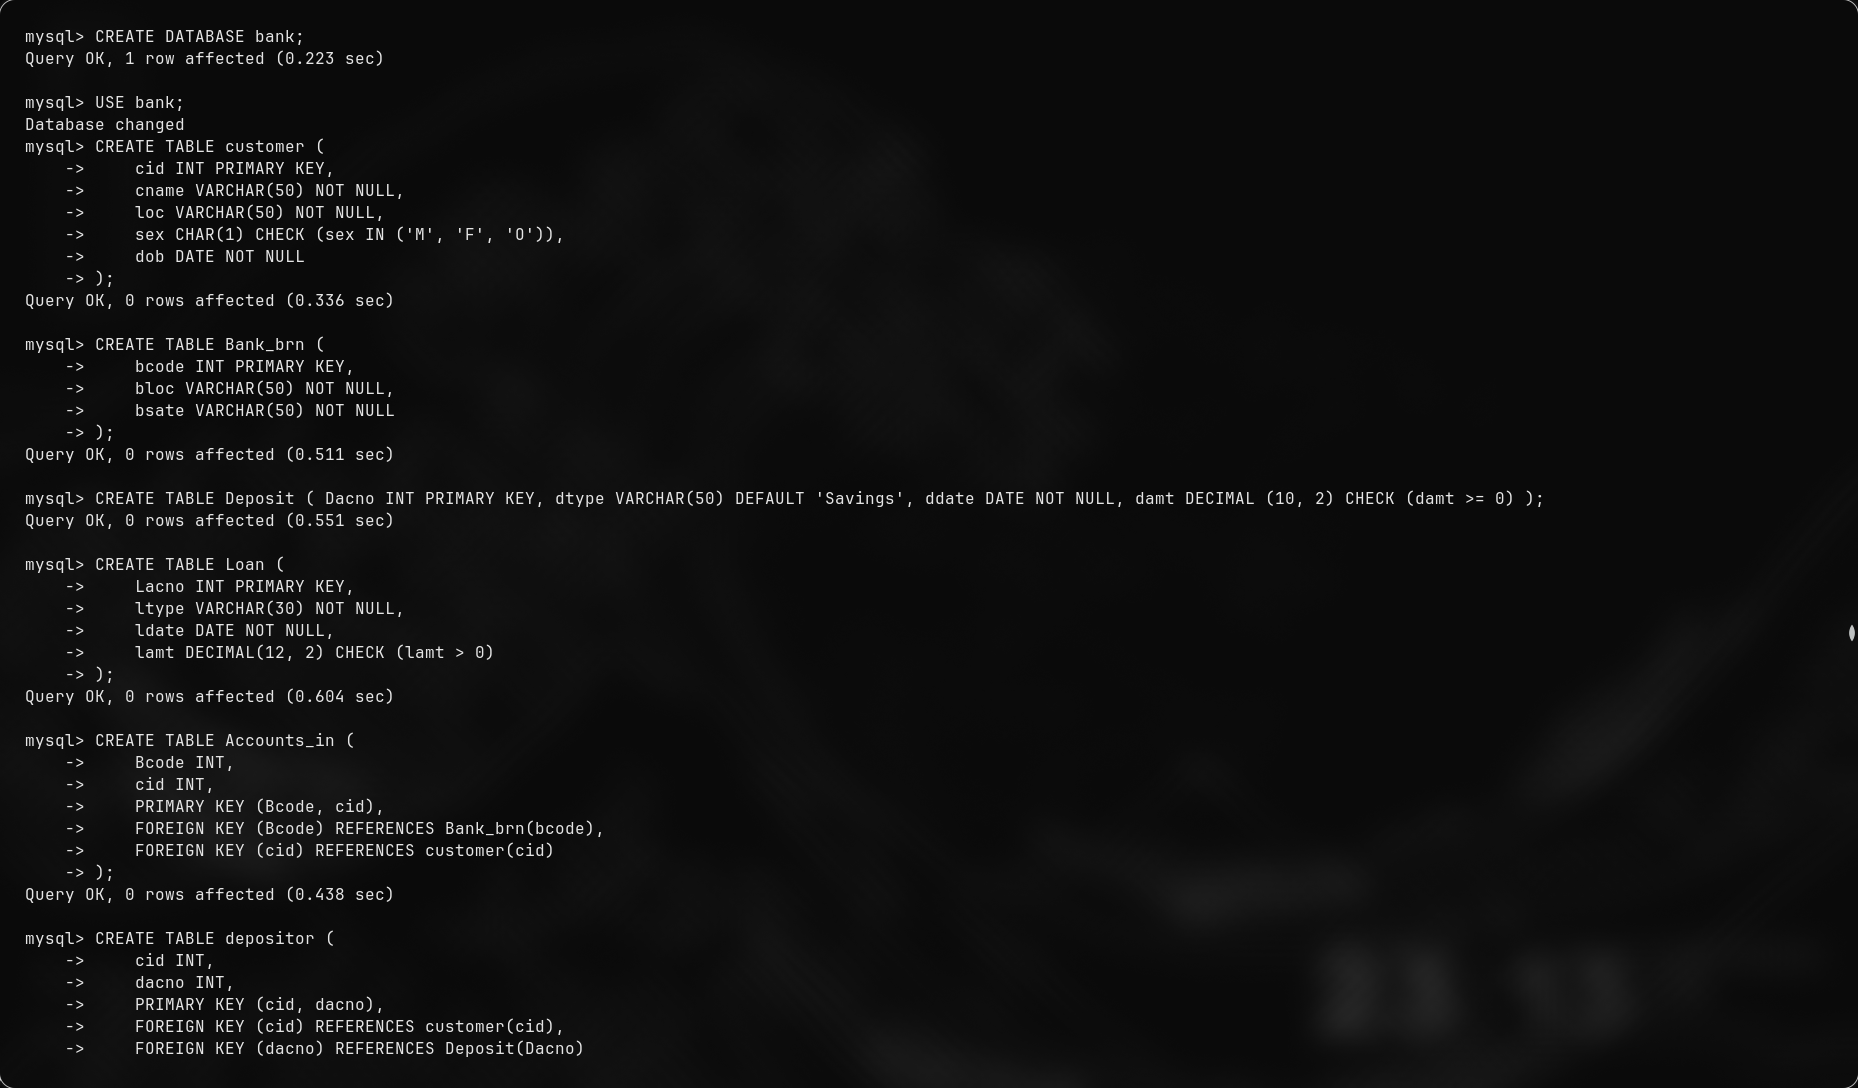
\includegraphics[width=0.92\linewidth,height=7.8cm,keepaspectratio]{Exp2-prob2-01.png}
    \caption{Database creation, active context selection, and creation of customer, Bank\_brn, Deposit, Loan, Accounts\_in.}
    \label{fig:exp2_bank_create1}
\end{figure}

\vspace{0.2cm}

\begin{figure}[H]
    \centering
    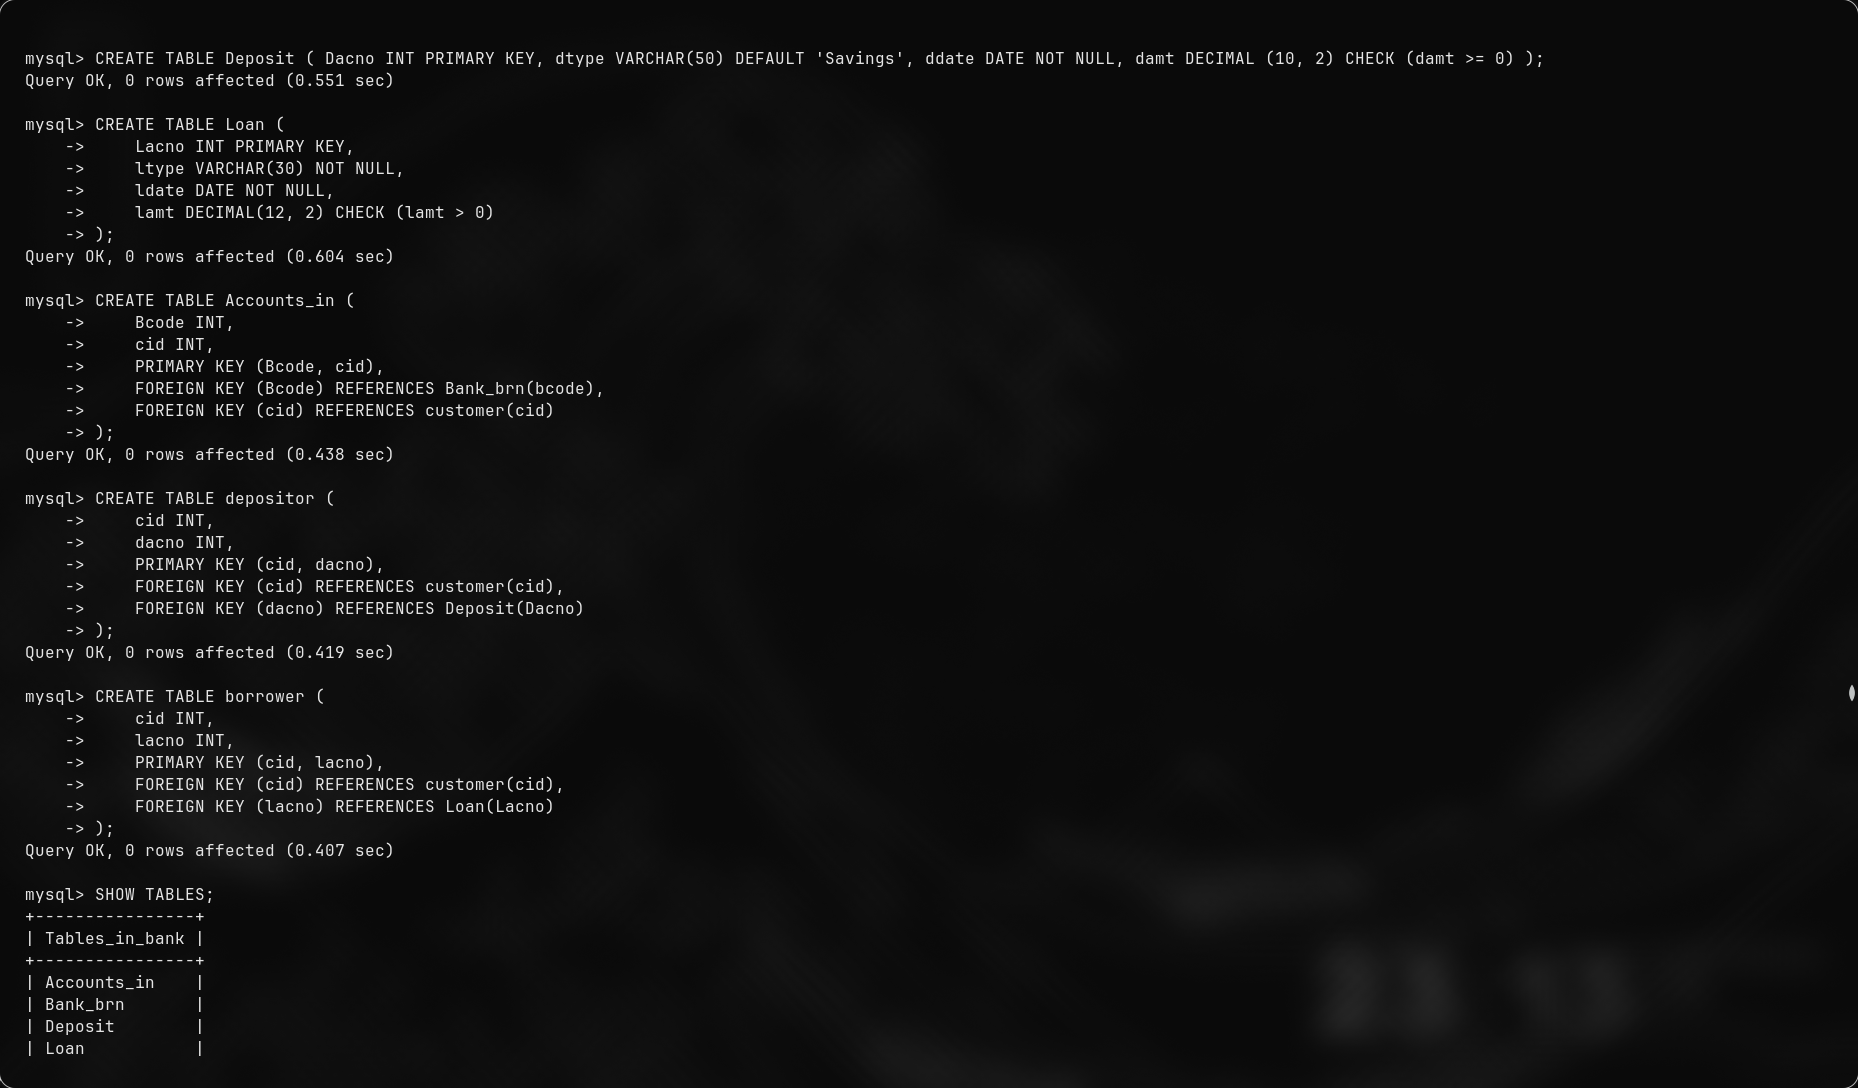
\includegraphics[width=0.92\linewidth,height=8.0cm,keepaspectratio]{Exp2-prob2-02.png}
    \caption{Creation of depositor and borrower tables with referential integrity constraints.}
    \label{fig:exp2_bank_create2}
\end{figure}

\newpage

\begin{figure}[H]
    \centering
    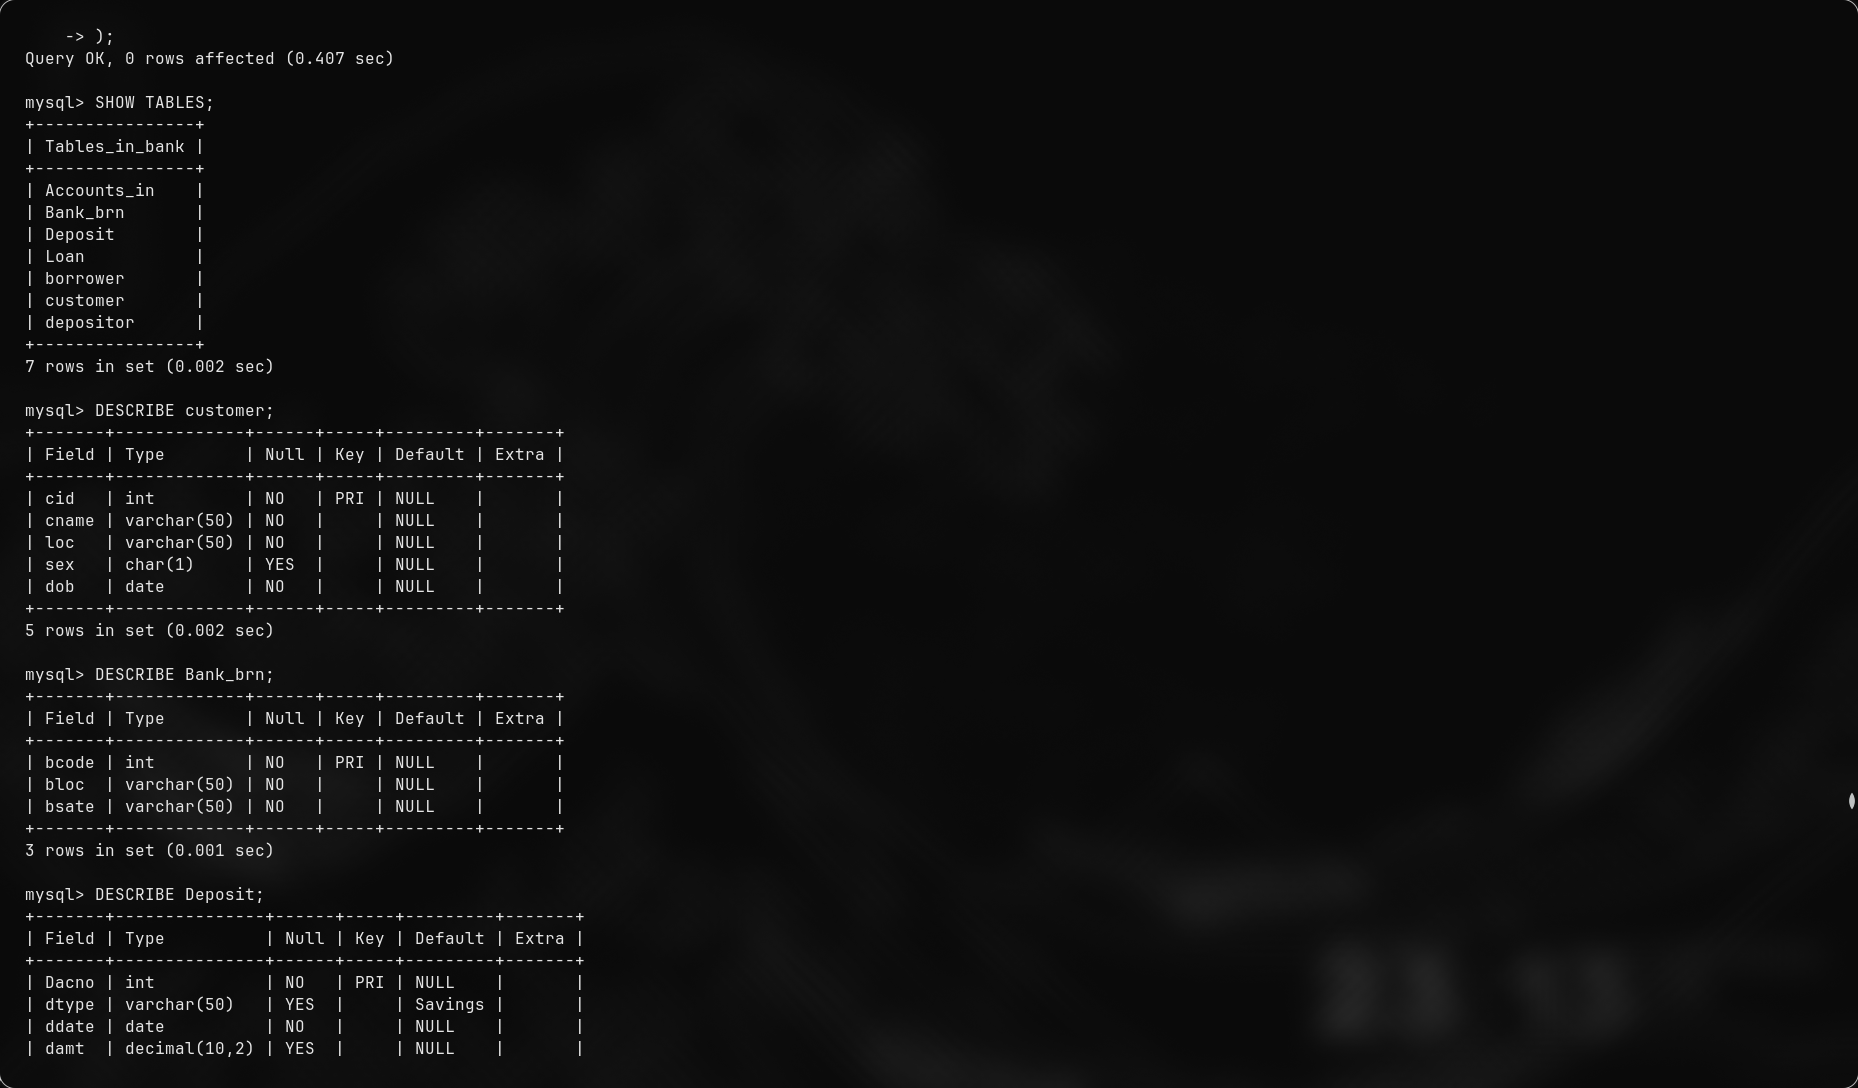
\includegraphics[width=0.92\linewidth,height=7.8cm,keepaspectratio]{Exp2-prob2-03.png}
    \caption{Verification of all seven tables via \texttt{SHOW TABLES;} and schema inspection of customer, Bank\_brn, Deposit.}
    \label{fig:exp2_bank_inspect1}
\end{figure}

\vspace{0.2cm}

\begin{figure}[H]
    \centering
    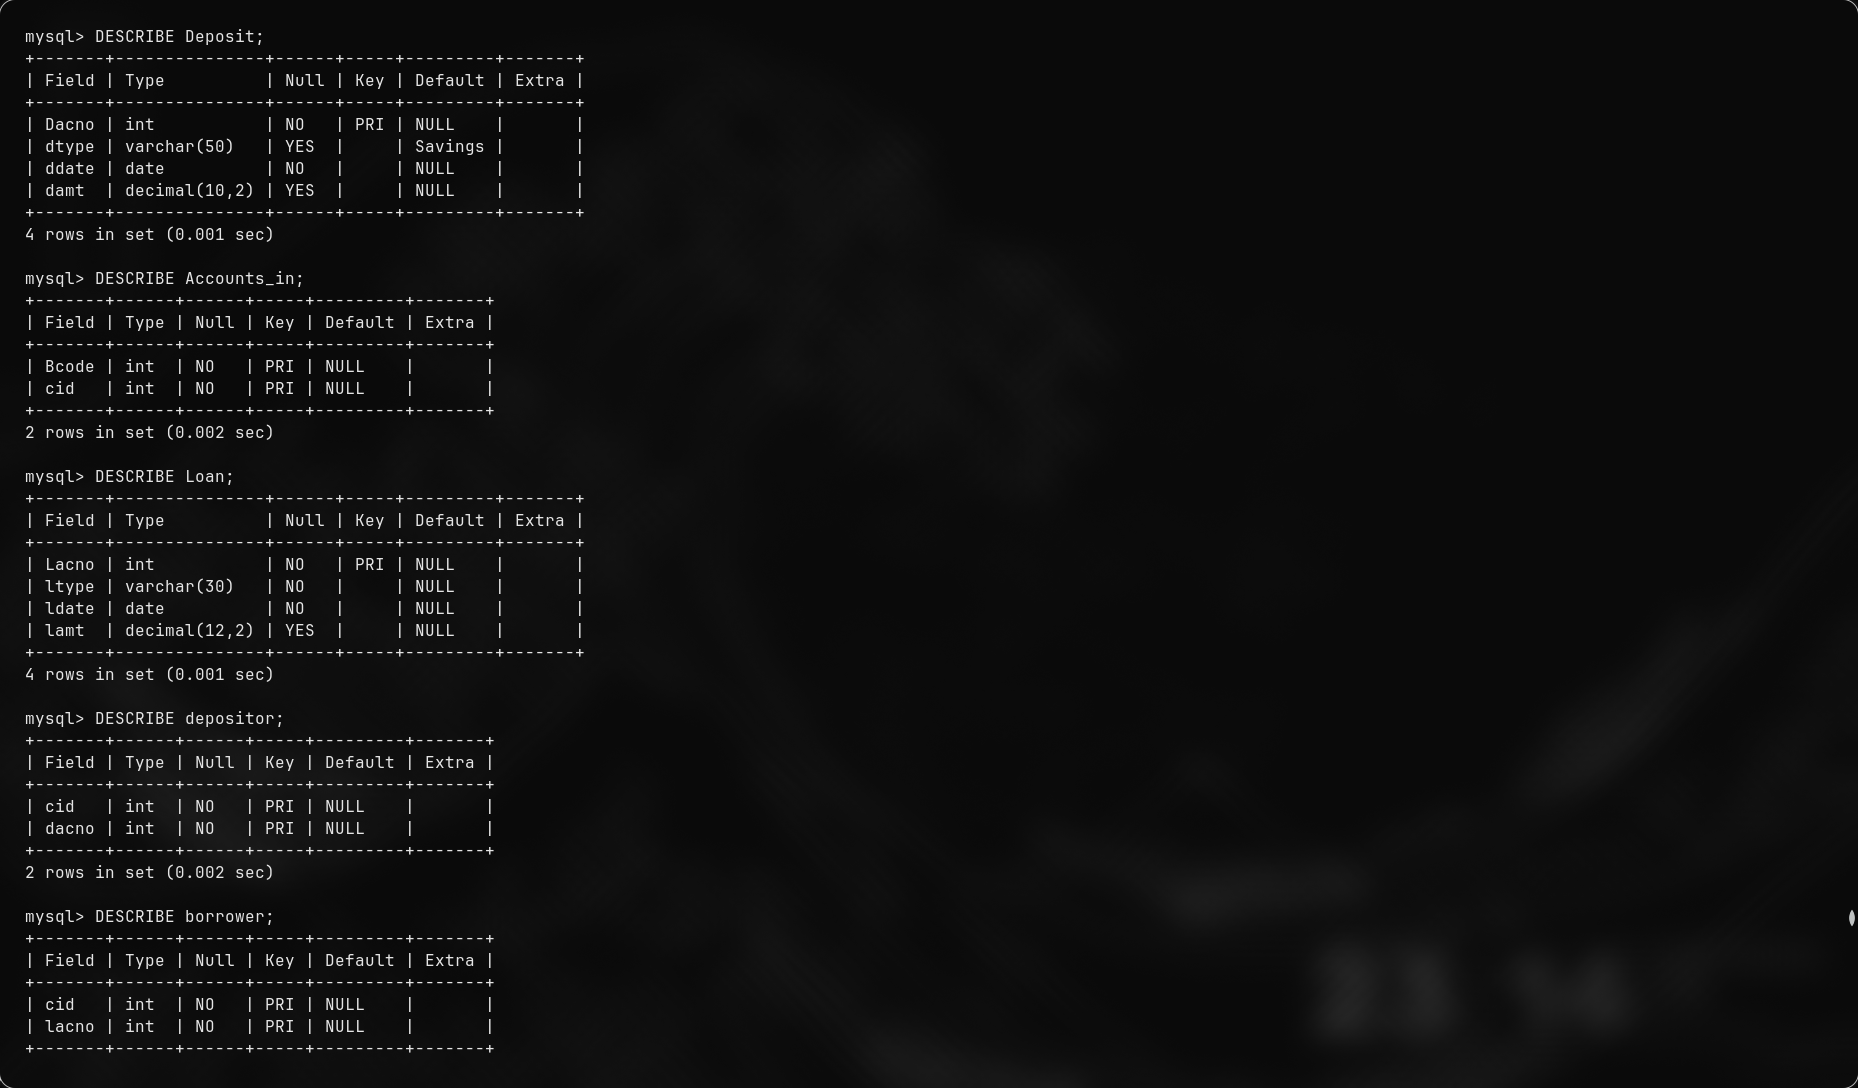
\includegraphics[width=0.92\linewidth,height=8.0cm,keepaspectratio]{Exp2-prob2-04.png}
    \caption{Schema inspection of Accounts\_in, Loan, depositor, and borrower tables.}
    \label{fig:exp2_bank_inspect2}
\end{figure}

\newpage

\begin{figure}[H]
    \centering
    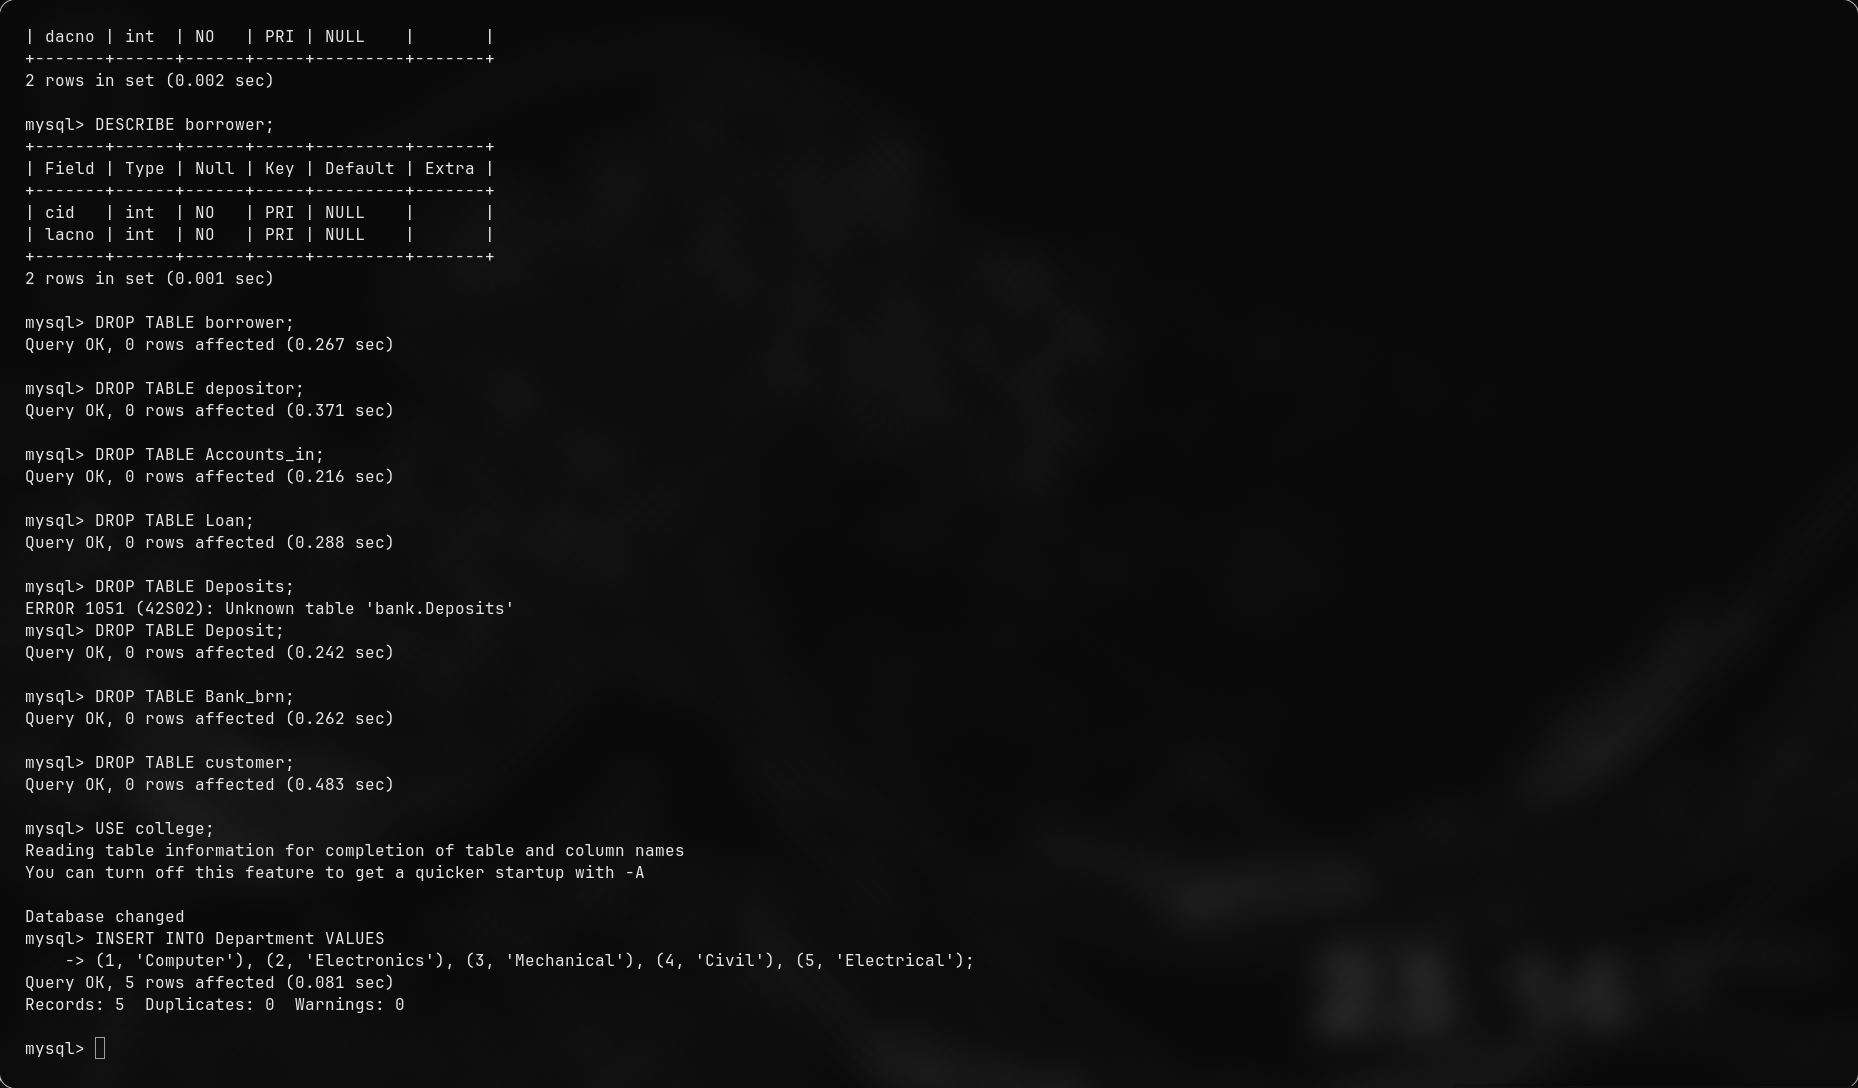
\includegraphics[width=0.92\linewidth,height=9.5cm,keepaspectratio]{Exp2-prob2-05.png}
    \caption{Final schema inspection and deletion of tables using \texttt{DROP TABLE} adhering to referential constraints.}
    \label{fig:exp2_bank_drop}
\end{figure}

\vspace{0.4cm}
\noindent\textbf{Result / Observation:}\quad The Data Definition Language (DDL) commands for the Banking Enterprise database were executed successfully in MySQL. All tables were created with proper primary key, foreign key, check, and default constraints. Schema structures were inspected via \texttt{DESCRIBE}, and tables were successfully dropped maintaining referential integrity.


\newpage

\section{Experiment 3: Data Manipulation Language (DML)}
\label{exp:dml}

\subsection*{Aim}
To populate, query, modify, and delete tuples in the \texttt{organisation} database using Data Manipulation Language (DML) commands in MySQL:
\begin{enumerate}[noitemsep,topsep=2pt]
    \item[(i)] Populate 5 rows each in \texttt{department} and \texttt{employee} tables and verify contents.
    \item[(ii)] Filter tuples by department, salary ranges (\texttt{BETWEEN}), and pattern conditions.
    \item[(iii)] Sort query results in descending order using \texttt{ORDER BY}.
    \item[(iv)] Eliminate duplicate records from queries using \texttt{DISTINCT}.
    \item[(v)] Compute aggregate summaries using \texttt{GROUP BY} and filter groups using \texttt{HAVING}.
    \item[(vi)] Modify records using \texttt{UPDATE} and remove specific tuples using \texttt{DELETE}.
\end{enumerate}

\subsection*{Objectives}
\begin{itemize}[noitemsep,topsep=2pt]
    \item To understand core DML statements: \texttt{INSERT}, \texttt{SELECT}, \texttt{UPDATE}, and \texttt{DELETE}.
    \item To construct targeted query predicates using \texttt{WHERE}, \texttt{BETWEEN}, and logical operators.
    \item To aggregate data and filter summarized groups using \texttt{GROUP BY} and \texttt{HAVING}.
\end{itemize}

\subsection*{Theory}
Data Manipulation Language (DML) enables retrieval and modification of records stored in relational tables.

\subsubsection*{1. Data Manipulation Statements}
\begin{itemize}[noitemsep,topsep=2pt]
    \item \textbf{INSERT:} Inserts new tuples into relational tables (\texttt{INSERT INTO}).
    \item \textbf{SELECT:} Queries and projects records based on predicates (\texttt{SELECT ... FROM}).
    \item \textbf{UPDATE:} Modifies existing column values in tuples (\texttt{UPDATE ... SET}).
    \item \textbf{DELETE:} Removes specific rows without altering schema (\texttt{DELETE FROM}).
\end{itemize}

\subsubsection*{2. Query Operators, Sorting, and Aggregations}
\begin{itemize}[noitemsep,topsep=2pt]
    \item \textbf{DISTINCT:} Eliminates duplicate tuples from query results (\texttt{SELECT DISTINCT}).
    \item \textbf{ORDER BY:} Orders output in ascending (\texttt{ASC}) or descending (\texttt{DESC}) order.
    \item \textbf{BETWEEN ... AND:} Tests whether an attribute falls within an inclusive numeric range.
    \item \textbf{GROUP BY \& HAVING:} \texttt{GROUP BY} partitions tuples into summary groups for aggregate functions (\texttt{SUM}, \texttt{AVG}), while \texttt{HAVING} filters these groups based on aggregate conditions.
\end{itemize}

\newpage

\subsection*{Commands Execution \& Output Screenshots}

\subsubsection*{Part 1: Inserting Tuples and Displaying Table Records}
Records are inserted into \texttt{department} followed by child tuples in \texttt{employee}. Both tables are subsequently verified:

\begin{lstlisting}[caption={Inserting rows into department and employee tables}]
USE organisation;

-- Insert records into department
INSERT INTO department (dept_no, dept_name) VALUES
(1, 'HR'), (2, 'Engineering'), (3, 'Finance'), (4, 'Marketing'), (5, 'Admin');

-- Insert records into employee
INSERT INTO employee VALUES
(101, 'Arun', '1997-04-10', 'Guwahati', '2022-05-01', '9876543210', 1, 15000, 'Developer'),
(102, 'John', '1998-05-14', 'Guwahati', '2022-01-10', '9876543211', 2, 22000, 'Developer'),
(103, 'Alice', '1995-08-20', 'Jorhat', '2021-03-15', '9876543212', 2, 35000, 'Manager'),
(104, 'Bob', '1999-11-30', 'Jorhat', '2023-06-01', '9876543213', 1, 10000, 'Typist'),
(105, 'Charlie', '1996-02-25', 'Tezpur', '2020-09-01', '9876543214', 3, 28000, 'Accountant');

SELECT * FROM department;
SELECT * FROM employee;
\end{lstlisting}

\begin{figure}[H]
    \centering
    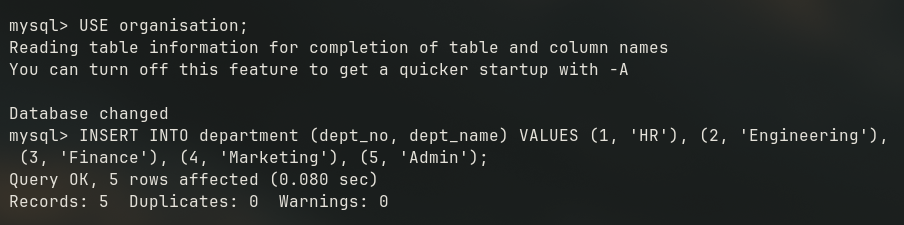
\includegraphics[width=0.88\linewidth,height=2.0cm,keepaspectratio]{Exp3-1.png}
    \caption{Populating tuples into the \texttt{department} table.}
    \label{fig:exp3_dept}
\end{figure}

\begin{figure}[H]
    \centering
    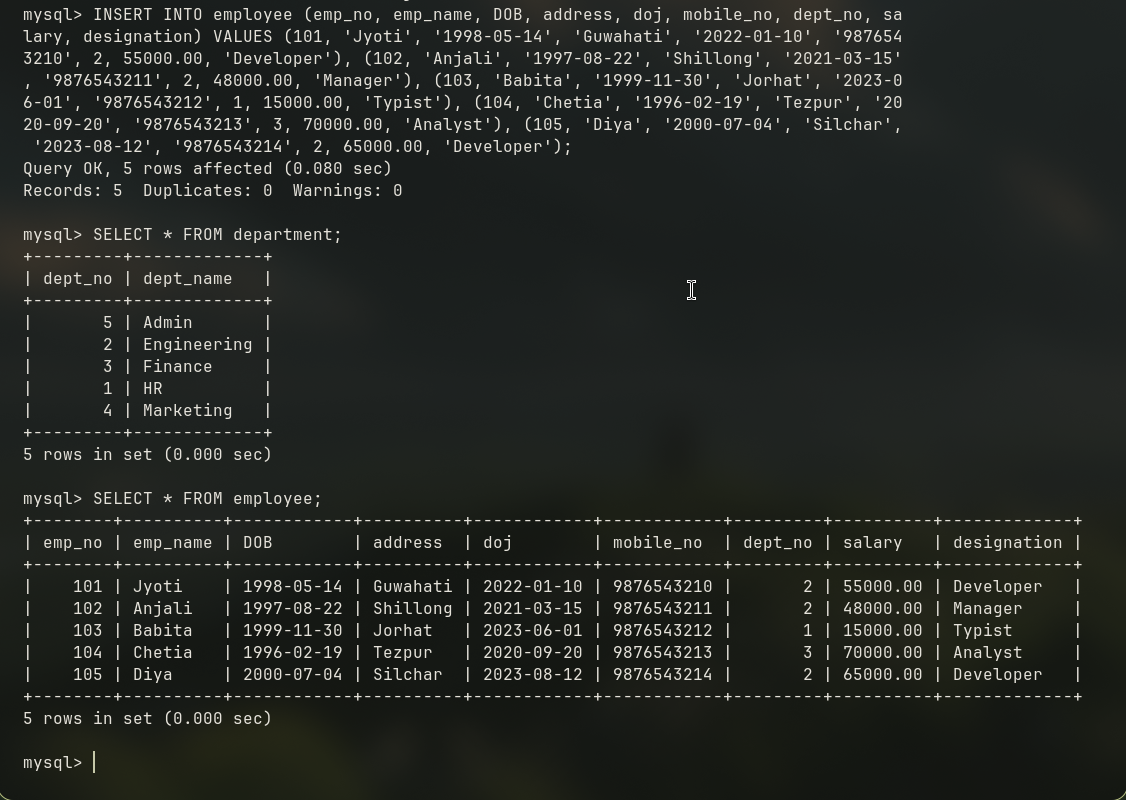
\includegraphics[width=0.88\linewidth,height=5.4cm,keepaspectratio]{Exp3-2.png}
    \caption{Populating tuples into the \texttt{employee} table and verifying records.}
    \label{fig:exp3_emp}
\end{figure}

\newpage

\subsubsection*{Part 2: Filtering, Sorting, Distinct, and Grouping Queries}
Queries filtering by department, sorting descending by salary, filtering ranges via \texttt{BETWEEN}, eliminating duplicate designations via \texttt{DISTINCT}, and grouping departmental expenditures:

\begin{lstlisting}[caption={Executing selective queries, sorting, distinct, and updates}]
-- Employees in Dept 2 and descending salary ordering
SELECT emp_no, emp_name FROM employee WHERE dept_no = 2;
SELECT emp_no, emp_name, designation, dept_no, salary FROM employee ORDER BY salary DESC;

-- Salary range filtering and distinct designations
SELECT emp_no, emp_name FROM employee WHERE salary BETWEEN 20000 AND 50000;
SELECT DISTINCT designation FROM employee;

-- Departmental expenditure and updating Typist salary
SELECT dept_no, SUM(salary) AS total_salary FROM employee GROUP BY dept_no;
UPDATE employee SET salary = 25000 WHERE designation = 'Typist';
\end{lstlisting}

\begin{figure}[H]
    \centering
    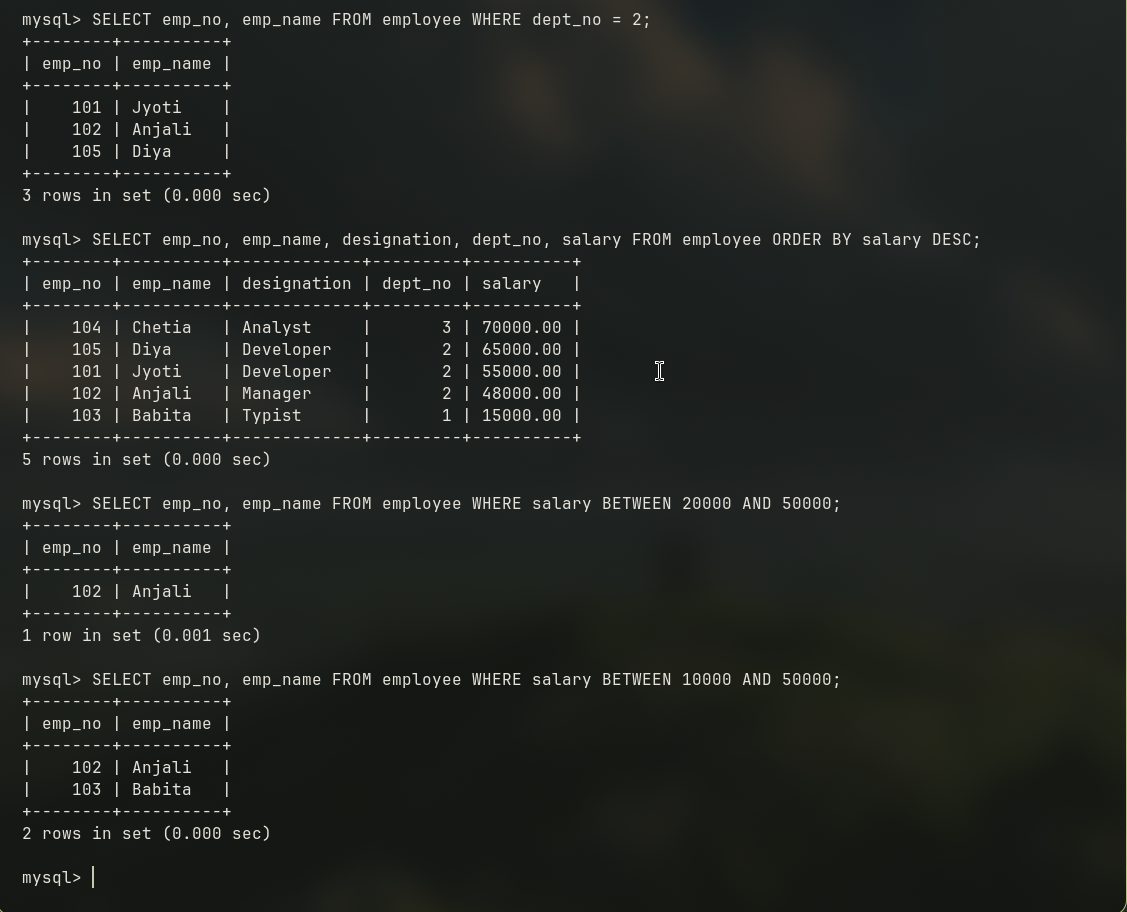
\includegraphics[width=0.88\linewidth,height=5.2cm,keepaspectratio]{Exp3-3.png}
    \caption{Filtering by department, descending sorting, and range condition queries.}
    \label{fig:exp3_filter}
\end{figure}

\begin{figure}[H]
    \centering
    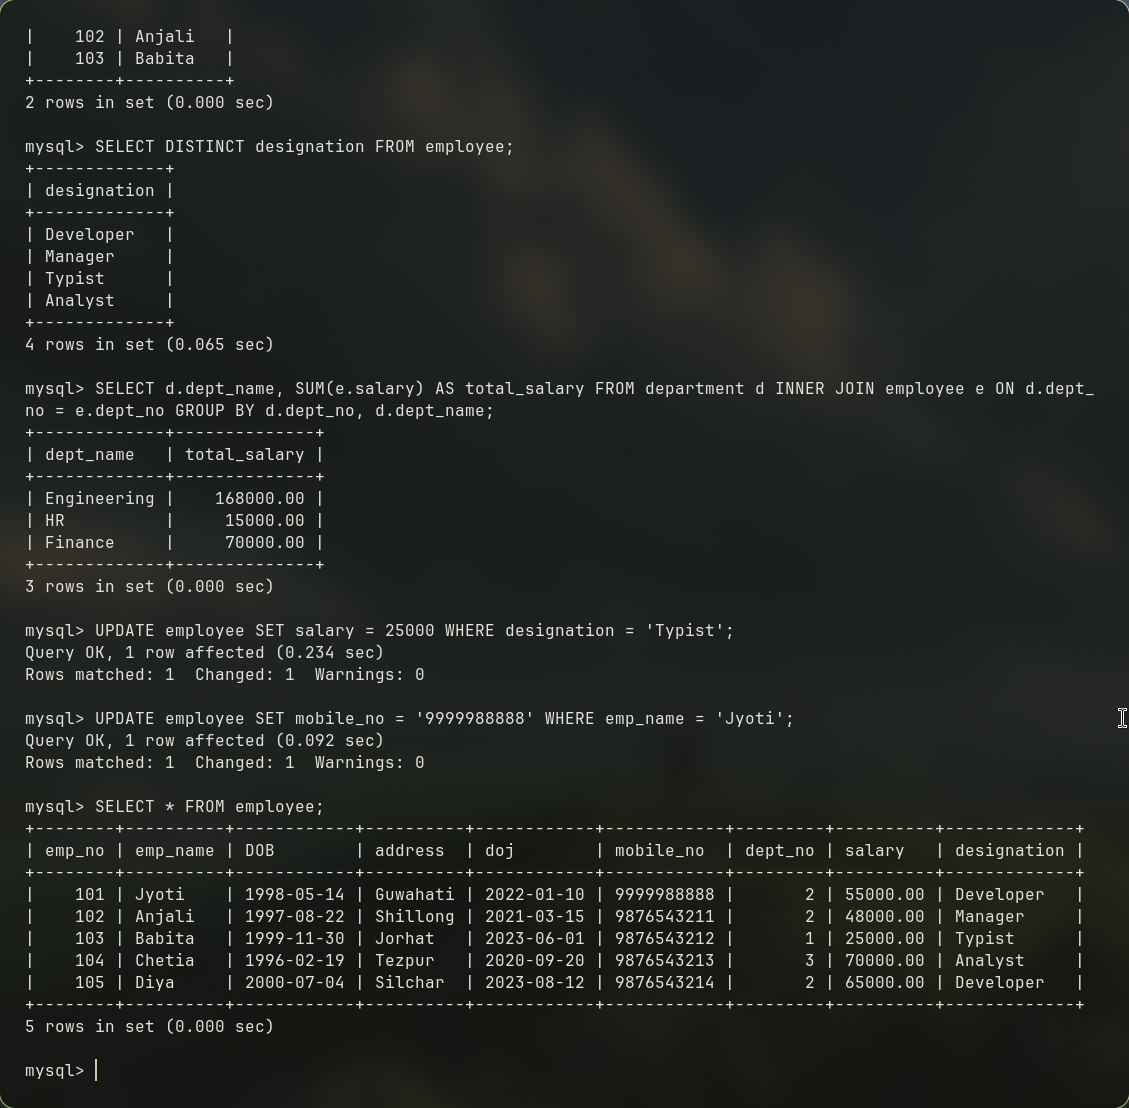
\includegraphics[width=0.88\linewidth,height=5.2cm,keepaspectratio]{Exp3-4.png}
    \caption{Distinct designations, grouped departmental summaries, and record modification.}
    \label{fig:exp3_group}
\end{figure}

\newpage

\subsubsection*{Part 3: Record Deletion and Filtered Group Aggregations}
Records matching a deletion predicate are removed using \texttt{DELETE}, and departments with aggregated salary expenditures exceeding 25,000 are queried using \texttt{HAVING}:

\begin{lstlisting}[caption={Executing DELETE and HAVING clause queries}]
-- Delete employees with salary equal to 70000
DELETE FROM employee WHERE salary = 70000;
SELECT * FROM employee;

-- Departments with total salary expenditure > 25000
SELECT dept_no, SUM(salary) AS total_salary 
FROM employee 
GROUP BY dept_no 
HAVING SUM(salary) > 25000;
\end{lstlisting}

\begin{figure}[H]
    \centering
    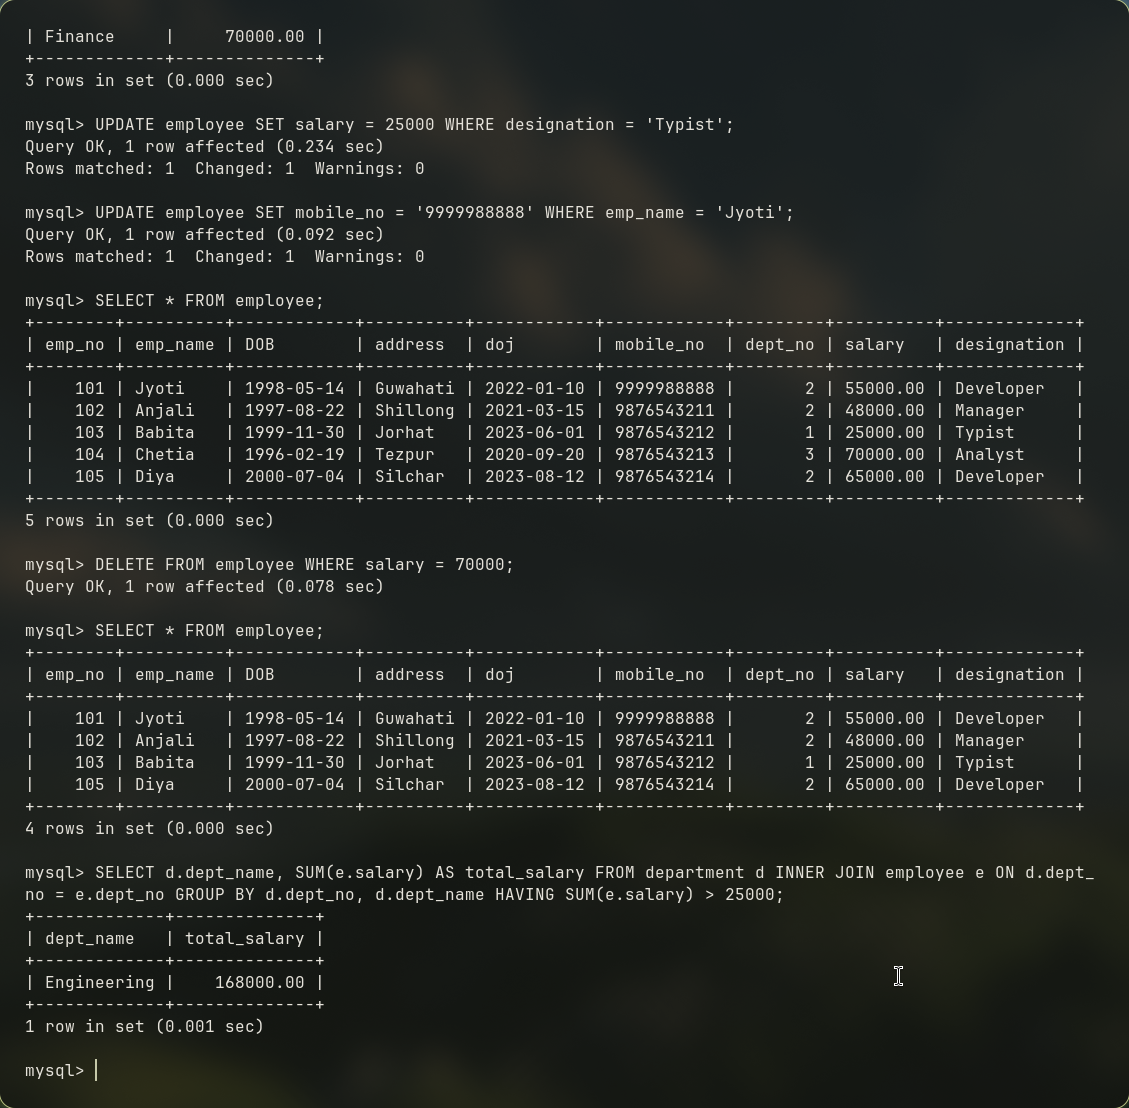
\includegraphics[width=0.88\linewidth,height=8.5cm,keepaspectratio]{Exp3-5.png}
    \caption{Tuple deletion verification and filtered group aggregations via \texttt{HAVING}.}
    \label{fig:exp3_delete_having}
\end{figure}

\subsection*{Result}
DML commands including record insertion, multi-criteria filtering, descending sorting, duplicate elimination, grouped aggregations, updates, and deletions were executed and verified successfully in MySQL.


\newpage

\label{exp:subqueries_joins}
\noindent
\begin{center}
    {\LARGE \textbf{DBMS LABORATORY PRACTICAL}}\\[0.25cm]
    \textbf{Practical No.:} 4 \hfill \textbf{Date:} 20/10/2026 \hfill \textbf{Page No.:} \thepage
\end{center}
\vspace{-0.2cm}
\hrule
\vspace{0.35cm}

\subsection*{Question / Problem Statement}
Design, implement, and execute nested subqueries and relational table joins on the \texttt{organisation} database using MySQL:
\begin{enumerate}[noitemsep,topsep=2pt]
    \item[(i)] Display employees earning more than the average salary.
    \item[(ii)] Display details of employees earning the minimum salary.
    \item[(iii)] Display all employees whose designation is identical to that of 'Arun'.
    \item[(iv)] Display employees who earn more than any employee in Department 1.
    \item[(v)] Display employee number, name, and department using \texttt{INNER JOIN}.
    \item[(vi)] Display employee details implementing a Left Outer Join (\texttt{LEFT OUTER JOIN}).
    \item[(vii)] Display employee details implementing a Right Outer Join (\texttt{RIGHT OUTER JOIN}).
\end{enumerate}

\vspace{0.25cm}
\subsection*{1. Single-Row Subqueries (Queries i, ii, iii)}

\subsubsection*{SQL Query}
\begin{lstlisting}[caption={Single-row subqueries using AVG, MIN, and attribute equality}]
USE organisation;

-- (i) Employees earning higher than the average salary
SELECT emp_no, emp_name, salary FROM employee
WHERE salary > (SELECT AVG(salary) FROM employee);

-- (ii) Details of employees earning the minimum salary
SELECT * FROM employee 
WHERE salary = (SELECT MIN(salary) FROM employee);

-- (iii) All employees sharing the same designation as 'Arun'
SELECT * FROM employee
WHERE designation = (
    SELECT designation FROM employee WHERE emp_name = 'Arun'
);
\end{lstlisting}

\newpage

\subsubsection*{Output Screenshot}
\begin{figure}[H]
    \centering
    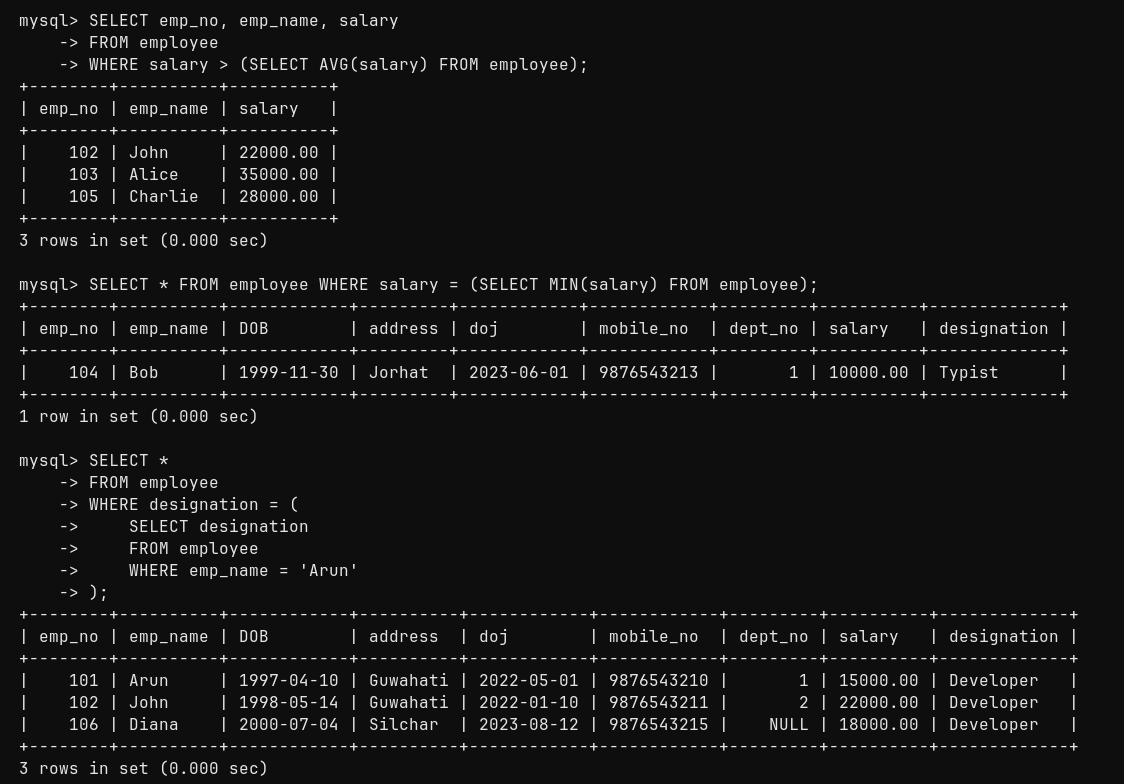
\includegraphics[width=0.92\linewidth,height=10.5cm,keepaspectratio]{Exp4-1.png}
    \caption{Single-row subqueries: employees above average salary, minimum salary, and matching designation.}
    \label{fig:exp4_subqueries_single}
\end{figure}

\newpage

\subsection*{2. Multi-Row Subquery \& Table Joins (Queries iv, v, vi, vii)}

\subsubsection*{SQL Query}
\begin{lstlisting}[caption={Multi-row subquery with ANY and table joins (INNER, LEFT, and RIGHT)}]
-- (iv) Employees earning more than any employee in Department 1
SELECT emp_no, emp_name FROM employee
WHERE salary > ANY (SELECT salary FROM employee WHERE dept_no = 1);
-- (v, vi) INNER JOIN and LEFT OUTER JOIN with department
SELECT e.emp_no, e.emp_name, d.dept_name
FROM employee e INNER JOIN department d ON e.dept_no = d.dept_no;
SELECT e.emp_no, e.emp_name, e.salary, d.dept_name
FROM employee e LEFT OUTER JOIN department d ON e.dept_no = d.dept_no;
-- (vii) RIGHT OUTER JOIN preserving unassigned departments
SELECT e.emp_no, e.emp_name, e.salary, d.dept_name
FROM employee e RIGHT OUTER JOIN department d ON e.dept_no = d.dept_no;
\end{lstlisting}

\subsubsection*{Output Screenshot}
\vspace{0.15cm}
\noindent\begin{minipage}[t]{0.48\textwidth}
    \centering
    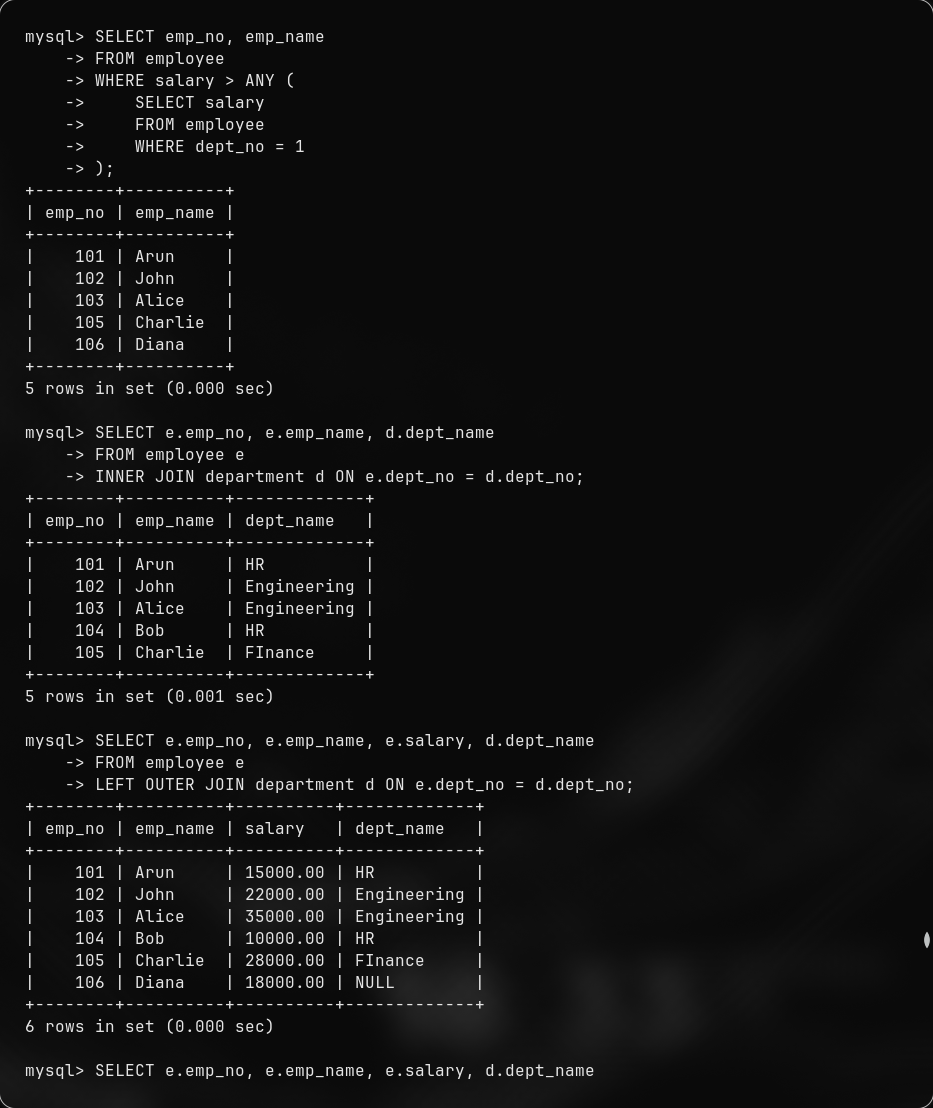
\includegraphics[width=\linewidth,height=7.2cm,keepaspectratio]{Exp4-2.png}
    \captionof{figure}{Queries iv, v, vi: \texttt{ANY}, Inner \& Left Join.}
    \label{fig:exp4_any_leftjoin}
\end{minipage}\hfill
\begin{minipage}[t]{0.48\textwidth}
    \centering
    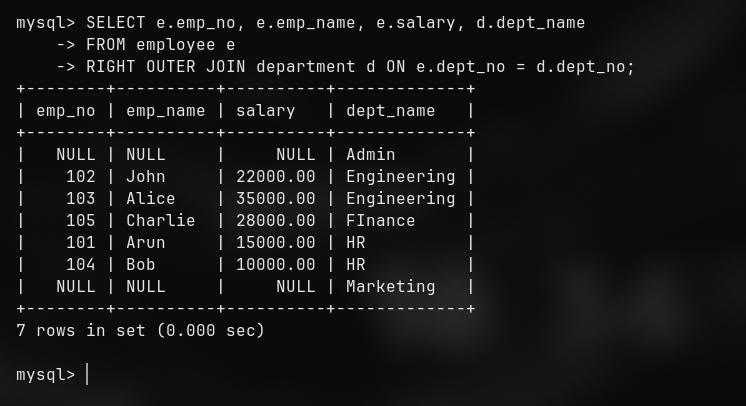
\includegraphics[width=\linewidth,height=4.2cm,keepaspectratio]{Exp4-3.png}
    \captionof{figure}{Query vii: Right Outer Join.}
    \label{fig:exp4_rightjoin}
\end{minipage}

\vspace{0.35cm}
\noindent\textbf{Result / Observation:}\quad The single-row subqueries, multi-row subqueries using \texttt{ANY}, and relational joins (\texttt{INNER JOIN}, \texttt{LEFT OUTER JOIN}, \texttt{RIGHT OUTER JOIN}) were executed successfully in MySQL.


\end{document}
